% Options for packages loaded elsewhere
\PassOptionsToPackage{unicode}{hyperref}
\PassOptionsToPackage{hyphens}{url}
\PassOptionsToPackage{dvipsnames,svgnames,x11names}{xcolor}
%
\documentclass[
  letterpaper,
  DIV=11,
  numbers=noendperiod]{scrreprt}

\usepackage{amsmath,amssymb}
\usepackage{lmodern}
\usepackage{iftex}
\ifPDFTeX
  \usepackage[T1]{fontenc}
  \usepackage[utf8]{inputenc}
  \usepackage{textcomp} % provide euro and other symbols
\else % if luatex or xetex
  \usepackage{unicode-math}
  \defaultfontfeatures{Scale=MatchLowercase}
  \defaultfontfeatures[\rmfamily]{Ligatures=TeX,Scale=1}
\fi
% Use upquote if available, for straight quotes in verbatim environments
\IfFileExists{upquote.sty}{\usepackage{upquote}}{}
\IfFileExists{microtype.sty}{% use microtype if available
  \usepackage[]{microtype}
  \UseMicrotypeSet[protrusion]{basicmath} % disable protrusion for tt fonts
}{}
\makeatletter
\@ifundefined{KOMAClassName}{% if non-KOMA class
  \IfFileExists{parskip.sty}{%
    \usepackage{parskip}
  }{% else
    \setlength{\parindent}{0pt}
    \setlength{\parskip}{6pt plus 2pt minus 1pt}}
}{% if KOMA class
  \KOMAoptions{parskip=half}}
\makeatother
\usepackage{xcolor}
\setlength{\emergencystretch}{3em} % prevent overfull lines
\setcounter{secnumdepth}{5}
% Make \paragraph and \subparagraph free-standing
\ifx\paragraph\undefined\else
  \let\oldparagraph\paragraph
  \renewcommand{\paragraph}[1]{\oldparagraph{#1}\mbox{}}
\fi
\ifx\subparagraph\undefined\else
  \let\oldsubparagraph\subparagraph
  \renewcommand{\subparagraph}[1]{\oldsubparagraph{#1}\mbox{}}
\fi

\usepackage{color}
\usepackage{fancyvrb}
\newcommand{\VerbBar}{|}
\newcommand{\VERB}{\Verb[commandchars=\\\{\}]}
\DefineVerbatimEnvironment{Highlighting}{Verbatim}{commandchars=\\\{\}}
% Add ',fontsize=\small' for more characters per line
\usepackage{framed}
\definecolor{shadecolor}{RGB}{241,243,245}
\newenvironment{Shaded}{\begin{snugshade}}{\end{snugshade}}
\newcommand{\AlertTok}[1]{\textcolor[rgb]{0.68,0.00,0.00}{#1}}
\newcommand{\AnnotationTok}[1]{\textcolor[rgb]{0.37,0.37,0.37}{#1}}
\newcommand{\AttributeTok}[1]{\textcolor[rgb]{0.40,0.45,0.13}{#1}}
\newcommand{\BaseNTok}[1]{\textcolor[rgb]{0.68,0.00,0.00}{#1}}
\newcommand{\BuiltInTok}[1]{\textcolor[rgb]{0.00,0.23,0.31}{#1}}
\newcommand{\CharTok}[1]{\textcolor[rgb]{0.13,0.47,0.30}{#1}}
\newcommand{\CommentTok}[1]{\textcolor[rgb]{0.37,0.37,0.37}{#1}}
\newcommand{\CommentVarTok}[1]{\textcolor[rgb]{0.37,0.37,0.37}{\textit{#1}}}
\newcommand{\ConstantTok}[1]{\textcolor[rgb]{0.56,0.35,0.01}{#1}}
\newcommand{\ControlFlowTok}[1]{\textcolor[rgb]{0.00,0.23,0.31}{#1}}
\newcommand{\DataTypeTok}[1]{\textcolor[rgb]{0.68,0.00,0.00}{#1}}
\newcommand{\DecValTok}[1]{\textcolor[rgb]{0.68,0.00,0.00}{#1}}
\newcommand{\DocumentationTok}[1]{\textcolor[rgb]{0.37,0.37,0.37}{\textit{#1}}}
\newcommand{\ErrorTok}[1]{\textcolor[rgb]{0.68,0.00,0.00}{#1}}
\newcommand{\ExtensionTok}[1]{\textcolor[rgb]{0.00,0.23,0.31}{#1}}
\newcommand{\FloatTok}[1]{\textcolor[rgb]{0.68,0.00,0.00}{#1}}
\newcommand{\FunctionTok}[1]{\textcolor[rgb]{0.28,0.35,0.67}{#1}}
\newcommand{\ImportTok}[1]{\textcolor[rgb]{0.00,0.46,0.62}{#1}}
\newcommand{\InformationTok}[1]{\textcolor[rgb]{0.37,0.37,0.37}{#1}}
\newcommand{\KeywordTok}[1]{\textcolor[rgb]{0.00,0.23,0.31}{#1}}
\newcommand{\NormalTok}[1]{\textcolor[rgb]{0.00,0.23,0.31}{#1}}
\newcommand{\OperatorTok}[1]{\textcolor[rgb]{0.37,0.37,0.37}{#1}}
\newcommand{\OtherTok}[1]{\textcolor[rgb]{0.00,0.23,0.31}{#1}}
\newcommand{\PreprocessorTok}[1]{\textcolor[rgb]{0.68,0.00,0.00}{#1}}
\newcommand{\RegionMarkerTok}[1]{\textcolor[rgb]{0.00,0.23,0.31}{#1}}
\newcommand{\SpecialCharTok}[1]{\textcolor[rgb]{0.37,0.37,0.37}{#1}}
\newcommand{\SpecialStringTok}[1]{\textcolor[rgb]{0.13,0.47,0.30}{#1}}
\newcommand{\StringTok}[1]{\textcolor[rgb]{0.13,0.47,0.30}{#1}}
\newcommand{\VariableTok}[1]{\textcolor[rgb]{0.07,0.07,0.07}{#1}}
\newcommand{\VerbatimStringTok}[1]{\textcolor[rgb]{0.13,0.47,0.30}{#1}}
\newcommand{\WarningTok}[1]{\textcolor[rgb]{0.37,0.37,0.37}{\textit{#1}}}

\providecommand{\tightlist}{%
  \setlength{\itemsep}{0pt}\setlength{\parskip}{0pt}}\usepackage{longtable,booktabs,array}
\usepackage{calc} % for calculating minipage widths
% Correct order of tables after \paragraph or \subparagraph
\usepackage{etoolbox}
\makeatletter
\patchcmd\longtable{\par}{\if@noskipsec\mbox{}\fi\par}{}{}
\makeatother
% Allow footnotes in longtable head/foot
\IfFileExists{footnotehyper.sty}{\usepackage{footnotehyper}}{\usepackage{footnote}}
\makesavenoteenv{longtable}
\usepackage{graphicx}
\makeatletter
\def\maxwidth{\ifdim\Gin@nat@width>\linewidth\linewidth\else\Gin@nat@width\fi}
\def\maxheight{\ifdim\Gin@nat@height>\textheight\textheight\else\Gin@nat@height\fi}
\makeatother
% Scale images if necessary, so that they will not overflow the page
% margins by default, and it is still possible to overwrite the defaults
% using explicit options in \includegraphics[width, height, ...]{}
\setkeys{Gin}{width=\maxwidth,height=\maxheight,keepaspectratio}
% Set default figure placement to htbp
\makeatletter
\def\fps@figure{htbp}
\makeatother
\newlength{\cslhangindent}
\setlength{\cslhangindent}{1.5em}
\newlength{\csllabelwidth}
\setlength{\csllabelwidth}{3em}
\newlength{\cslentryspacingunit} % times entry-spacing
\setlength{\cslentryspacingunit}{\parskip}
\newenvironment{CSLReferences}[2] % #1 hanging-ident, #2 entry spacing
 {% don't indent paragraphs
  \setlength{\parindent}{0pt}
  % turn on hanging indent if param 1 is 1
  \ifodd #1
  \let\oldpar\par
  \def\par{\hangindent=\cslhangindent\oldpar}
  \fi
  % set entry spacing
  \setlength{\parskip}{#2\cslentryspacingunit}
 }%
 {}
\usepackage{calc}
\newcommand{\CSLBlock}[1]{#1\hfill\break}
\newcommand{\CSLLeftMargin}[1]{\parbox[t]{\csllabelwidth}{#1}}
\newcommand{\CSLRightInline}[1]{\parbox[t]{\linewidth - \csllabelwidth}{#1}\break}
\newcommand{\CSLIndent}[1]{\hspace{\cslhangindent}#1}

\usepackage{booktabs}
\usepackage{longtable}
\usepackage{array}
\usepackage{multirow}
\usepackage{wrapfig}
\usepackage{float}
\usepackage{colortbl}
\usepackage{pdflscape}
\usepackage{tabu}
\usepackage{threeparttable}
\usepackage{threeparttablex}
\usepackage[normalem]{ulem}
\usepackage{makecell}
\usepackage{xcolor}
\KOMAoption{captions}{tableheading}
\makeatletter
\@ifpackageloaded{tcolorbox}{}{\usepackage[many]{tcolorbox}}
\@ifpackageloaded{fontawesome5}{}{\usepackage{fontawesome5}}
\definecolor{quarto-callout-color}{HTML}{909090}
\definecolor{quarto-callout-note-color}{HTML}{0758E5}
\definecolor{quarto-callout-important-color}{HTML}{CC1914}
\definecolor{quarto-callout-warning-color}{HTML}{EB9113}
\definecolor{quarto-callout-tip-color}{HTML}{00A047}
\definecolor{quarto-callout-caution-color}{HTML}{FC5300}
\definecolor{quarto-callout-color-frame}{HTML}{acacac}
\definecolor{quarto-callout-note-color-frame}{HTML}{4582ec}
\definecolor{quarto-callout-important-color-frame}{HTML}{d9534f}
\definecolor{quarto-callout-warning-color-frame}{HTML}{f0ad4e}
\definecolor{quarto-callout-tip-color-frame}{HTML}{02b875}
\definecolor{quarto-callout-caution-color-frame}{HTML}{fd7e14}
\makeatother
\makeatletter
\makeatother
\makeatletter
\@ifpackageloaded{bookmark}{}{\usepackage{bookmark}}
\makeatother
\makeatletter
\@ifpackageloaded{caption}{}{\usepackage{caption}}
\AtBeginDocument{%
\ifdefined\contentsname
  \renewcommand*\contentsname{Table of contents}
\else
  \newcommand\contentsname{Table of contents}
\fi
\ifdefined\listfigurename
  \renewcommand*\listfigurename{List of Figures}
\else
  \newcommand\listfigurename{List of Figures}
\fi
\ifdefined\listtablename
  \renewcommand*\listtablename{List of Tables}
\else
  \newcommand\listtablename{List of Tables}
\fi
\ifdefined\figurename
  \renewcommand*\figurename{Figure}
\else
  \newcommand\figurename{Figure}
\fi
\ifdefined\tablename
  \renewcommand*\tablename{Table}
\else
  \newcommand\tablename{Table}
\fi
}
\@ifpackageloaded{float}{}{\usepackage{float}}
\floatstyle{ruled}
\@ifundefined{c@chapter}{\newfloat{codelisting}{h}{lop}}{\newfloat{codelisting}{h}{lop}[chapter]}
\floatname{codelisting}{Listing}
\newcommand*\listoflistings{\listof{codelisting}{List of Listings}}
\makeatother
\makeatletter
\@ifpackageloaded{caption}{}{\usepackage{caption}}
\@ifpackageloaded{subcaption}{}{\usepackage{subcaption}}
\makeatother
\makeatletter
\@ifpackageloaded{tcolorbox}{}{\usepackage[many]{tcolorbox}}
\makeatother
\makeatletter
\@ifundefined{shadecolor}{\definecolor{shadecolor}{rgb}{.97, .97, .97}}
\makeatother
\makeatletter
\makeatother
\ifLuaTeX
  \usepackage{selnolig}  % disable illegal ligatures
\fi
\IfFileExists{bookmark.sty}{\usepackage{bookmark}}{\usepackage{hyperref}}
\IfFileExists{xurl.sty}{\usepackage{xurl}}{} % add URL line breaks if available
\urlstyle{same} % disable monospaced font for URLs
\hypersetup{
  pdftitle={Curso: Geoanálisis},
  pdfauthor={Denis Berroeta González (denis.berroeta@uai.cl)},
  colorlinks=true,
  linkcolor={blue},
  filecolor={Maroon},
  citecolor={Blue},
  urlcolor={Blue},
  pdfcreator={LaTeX via pandoc}}

\title{Curso: Geoanálisis}
\usepackage{etoolbox}
\makeatletter
\providecommand{\subtitle}[1]{% add subtitle to \maketitle
  \apptocmd{\@title}{\par {\large #1 \par}}{}{}
}
\makeatother
\subtitle{Diplomado en Ciencia de Datos para Políticas Públicas 2022}
\author{Denis Berroeta González (denis.berroeta@uai.cl)}
\date{2022-08-12}

\begin{document}
\maketitle
\ifdefined\Shaded\renewenvironment{Shaded}{\begin{tcolorbox}[borderline west={3pt}{0pt}{shadecolor}, enhanced, frame hidden, interior hidden, breakable, sharp corners, boxrule=0pt]}{\end{tcolorbox}}\fi

\renewcommand*\contentsname{Table of contents}
{
\hypersetup{linkcolor=}
\setcounter{tocdepth}{2}
\tableofcontents
}
\bookmarksetup{startatroot}

\hypertarget{antecedentes}{%
\chapter*{Antecedentes}\label{antecedentes}}
\addcontentsline{toc}{chapter}{Antecedentes}

Este libro corresponde al material de estudio del curso de Geoanálisis
del Diplomado en Ciencia de Datos para Políticas Públicas 2022, dictado
por Escuela de Gobierno de la Universidad Adolfo Ibáñez.

\hypertarget{introducciuxf3n}{%
\section*{Introducción}\label{introducciuxf3n}}
\addcontentsline{toc}{section}{Introducción}

Este curso se enfoca en entregar a los alumnos conocimientos teóricos y
herramientas técnicas para realizar análisis espacial de variables
territoriales en diferentes campos de aplicación, con énfasis en
afrontar desafíos relacionado a las políticas públicas, haciendo uso de
lenguaje de programación R Project, para uso de metodologías de alto
nivel y de forma automatizada.

\hypertarget{objetivos}{%
\section*{Objetivos}\label{objetivos}}
\addcontentsline{toc}{section}{Objetivos}

El objetivo general es proporcionar a los estudiantes los fundamentos,
técnicas y aspectos básicos para analizar, modelar y representar
información espacial, para apoyar la toma de decisiones con evidencia
territorial robusta.

Los objetivos específicos son:

\begin{itemize}
\tightlist
\item
  Conocer los conceptos básicos del geoanálisis.
\item
  Manipular datos espaciales en R.
\item
  Conocer técnicas de inferencia, autocorrelación y regresión espacial.
\item
  Aplicar las técnicas a problemas de interés público.
\end{itemize}

\hypertarget{modulos}{%
\section*{Modulos}\label{modulos}}
\addcontentsline{toc}{section}{Modulos}

\begin{figure}

{\centering 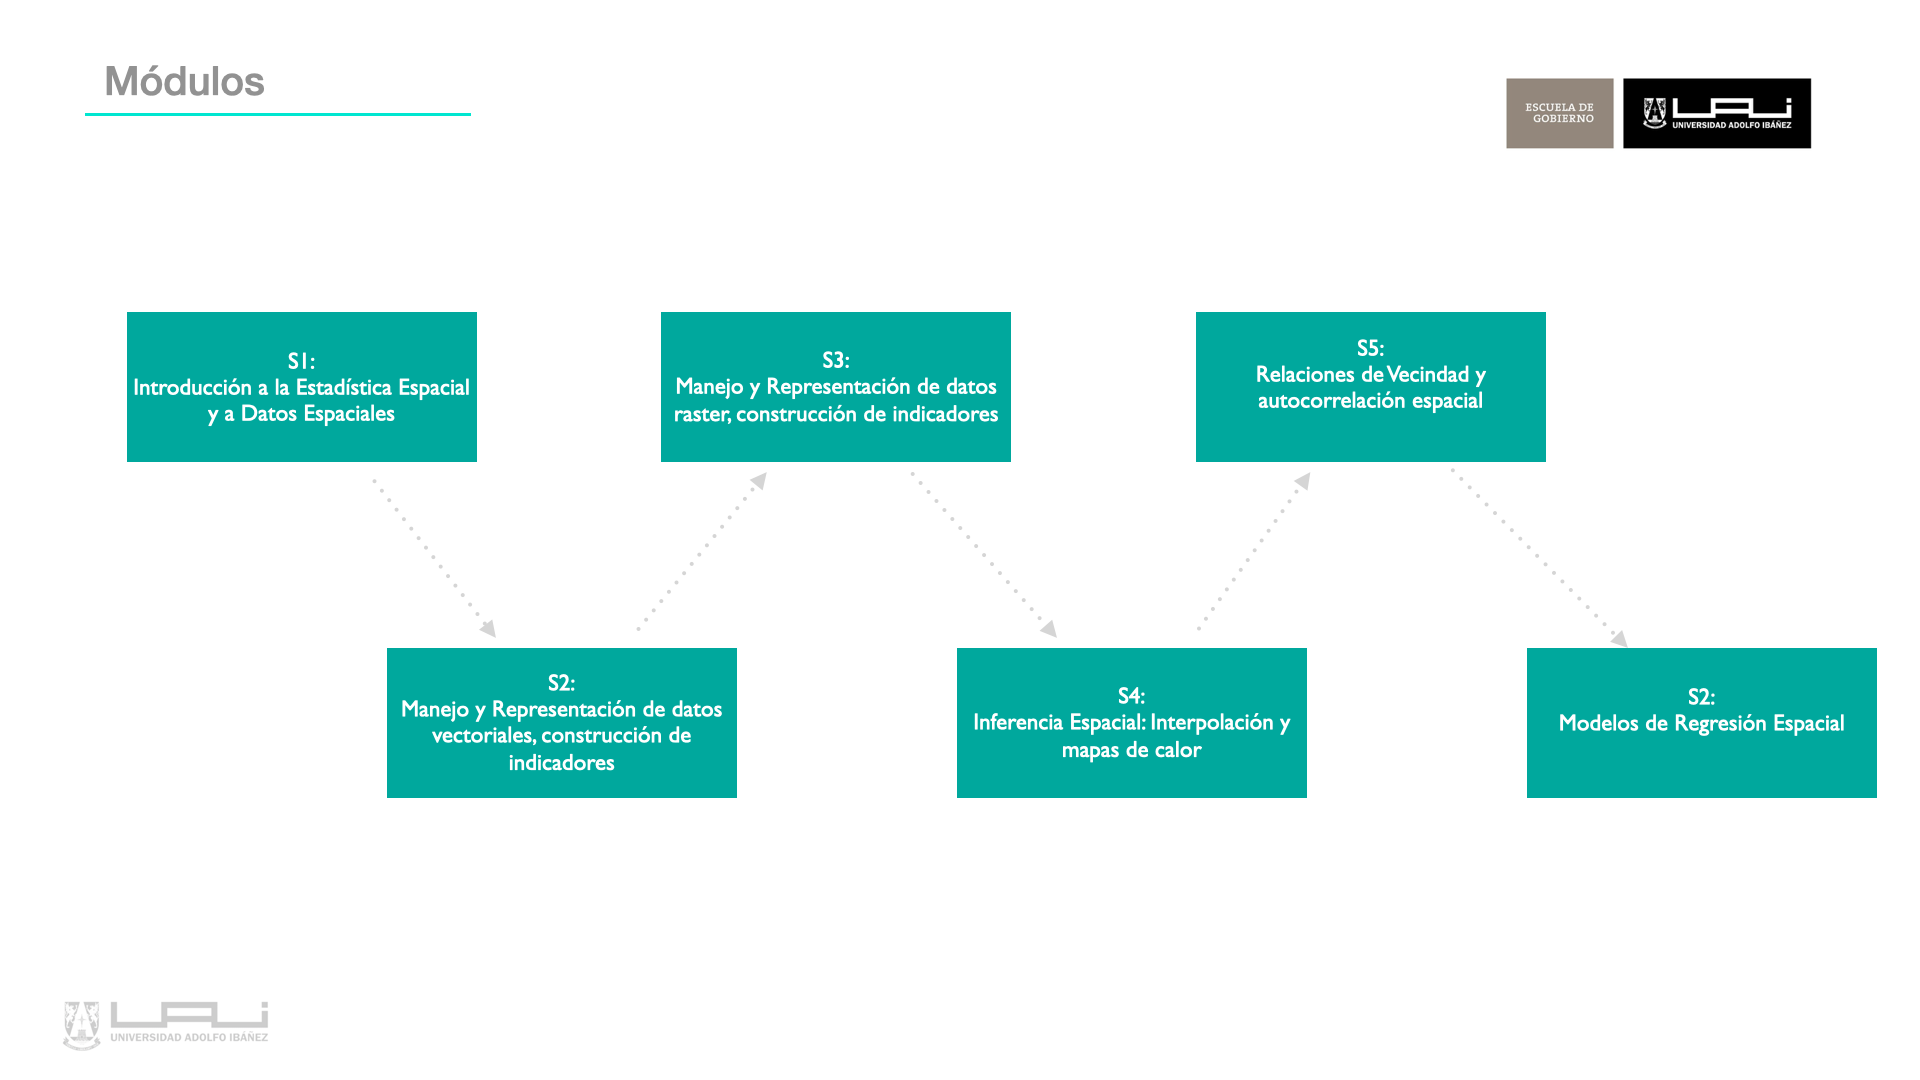
\includegraphics{./images/modulos.png}

}

\caption{Modulos}

\end{figure}

\begin{enumerate}
\def\labelenumi{\arabic{enumi}.}
\tightlist
\item
  Introducción a la Estadística Espacial y a Datos Espaciales
\item
  Manejo y Representación de datos vectoriales, construcción de
  indicadores
\item
  Manejo y Representación de datos raster, construcción de indicadores
\item
  Inferencia Espacial: Interpolación y mapas de calor
\item
  Relaciones de Vecindad y autocorrelación espacial
\item
  Modelos de Regresión Espacial
\end{enumerate}

\hypertarget{docentes}{%
\section*{Docentes}\label{docentes}}
\addcontentsline{toc}{section}{Docentes}

\begin{description}
\tightlist
\item[Profesor:]
Denis Berroeta González (denis.berroeta@uai.cl)
\end{description}

\begin{itemize}
\tightlist
\item
  Coordinador de Investigación Centro de Inteligencia Territorial UAI
\item
  Magister en Inteligencia Artificial FIC-UAI
\item
  Master of Data Science FIC-UAI (cursando)
\item
  Ingeniero en Prevención en Riesgos
\end{itemize}

\begin{description}
\tightlist
\item[Ayudante:]
Leonardo Rojas (leonardo.rojas@uai.cl)
\end{description}

\begin{itemize}
\tightlist
\item
  Analista Centro de Inteligencia Territorial UAI
\item
  Economista
\item
  Master of Data Science FIC-UAI (cursando)
\end{itemize}

\bookmarksetup{startatroot}

\hypertarget{introducciuxf3n-estaduxedstica-espacial}{%
\chapter{Introducción Estadística
Espacial}\label{introducciuxf3n-estaduxedstica-espacial}}

Módulo 1: Teórico

\hfill\break

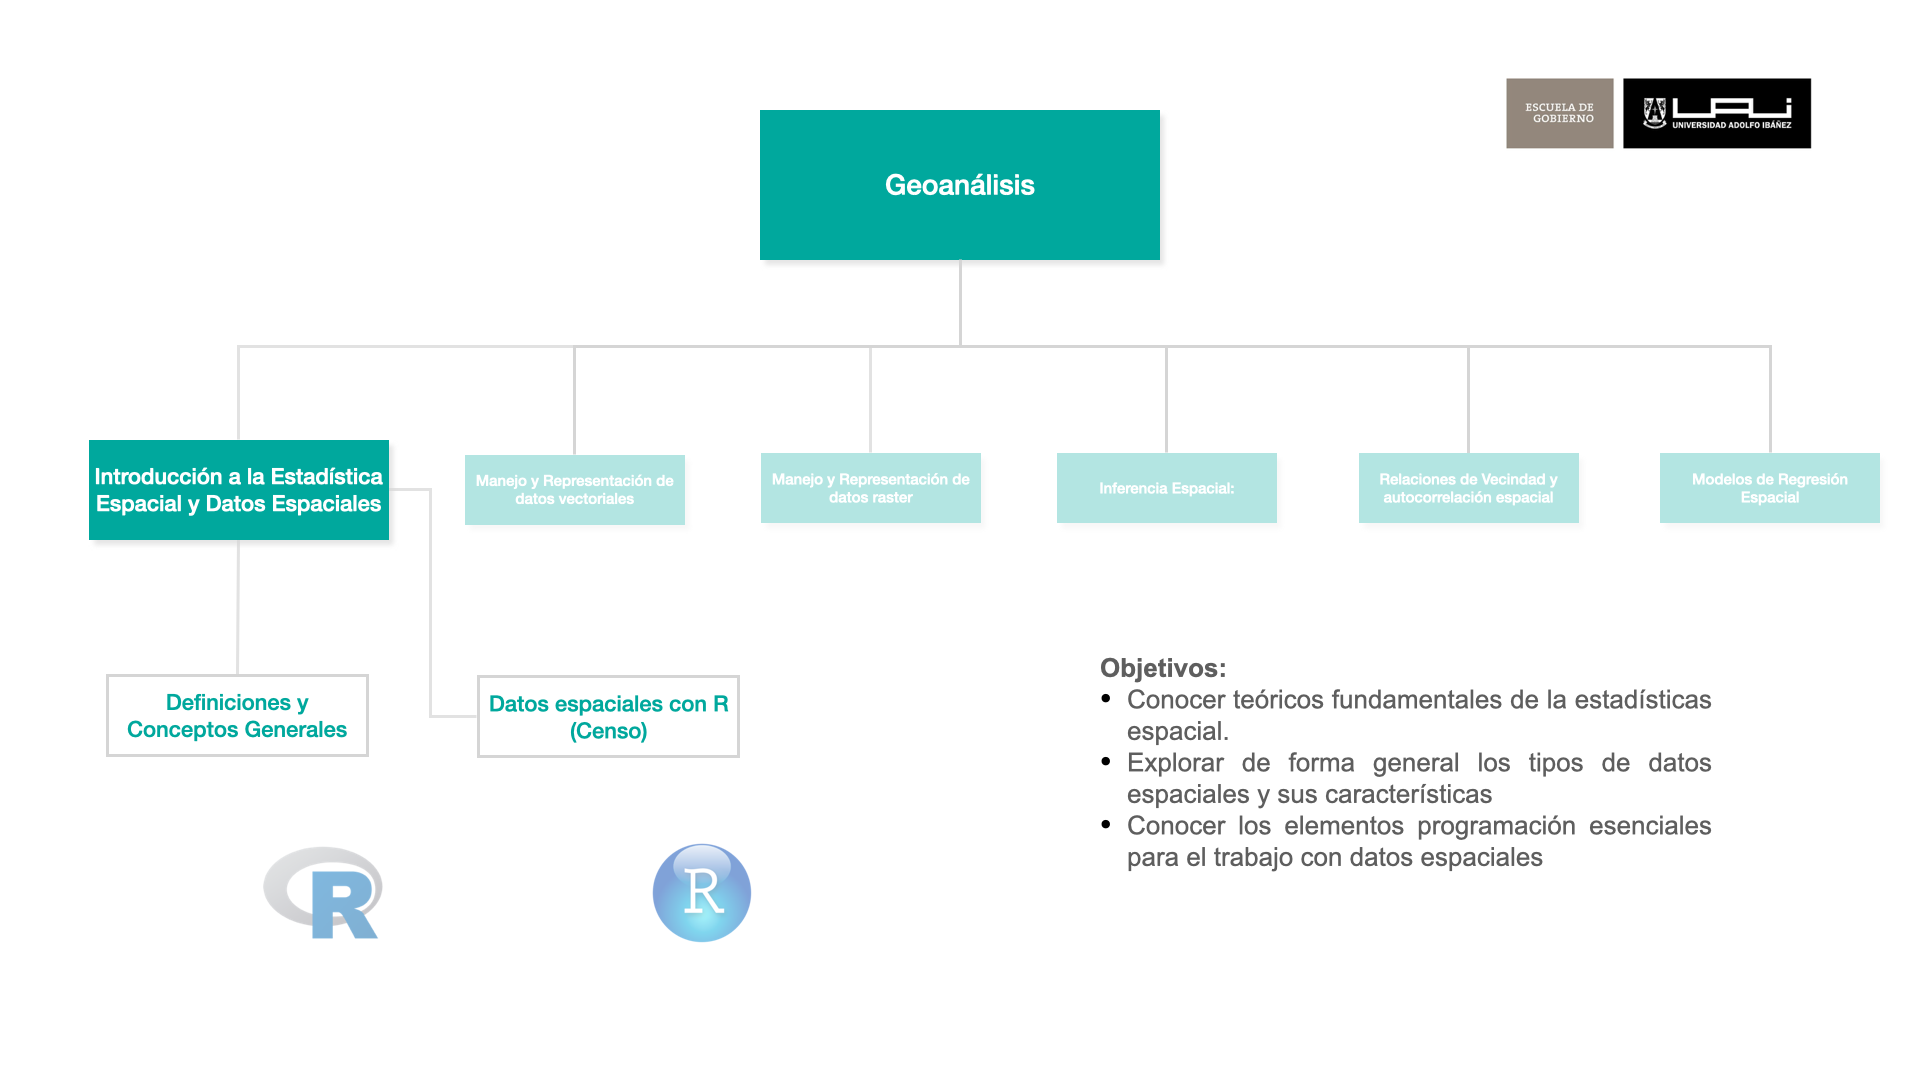
\includegraphics{./images/m1_objetivos.png} * Conocer teóricos
fundamentales de la estadística espacial.

\hypertarget{origen-de-la-estaduxedstica}{%
\section{Origen de la Estadística}\label{origen-de-la-estaduxedstica}}

Estadística deriva del italiano statista (hombre de Estado) y se
desarrolla desde la antigüedad para facilitar la gestión tributaria y
estimar la capacidad bélica de un reino. Ej: censos egipcios desde el
3050 a.C.

Durante la expansión de los imperios coloniales (siglos XVI - XIX) se
desarrolla la estadística en estrecha relación con la cartografía,
principalmente para la administración y dominio de territorios.

\begin{figure}

{\centering 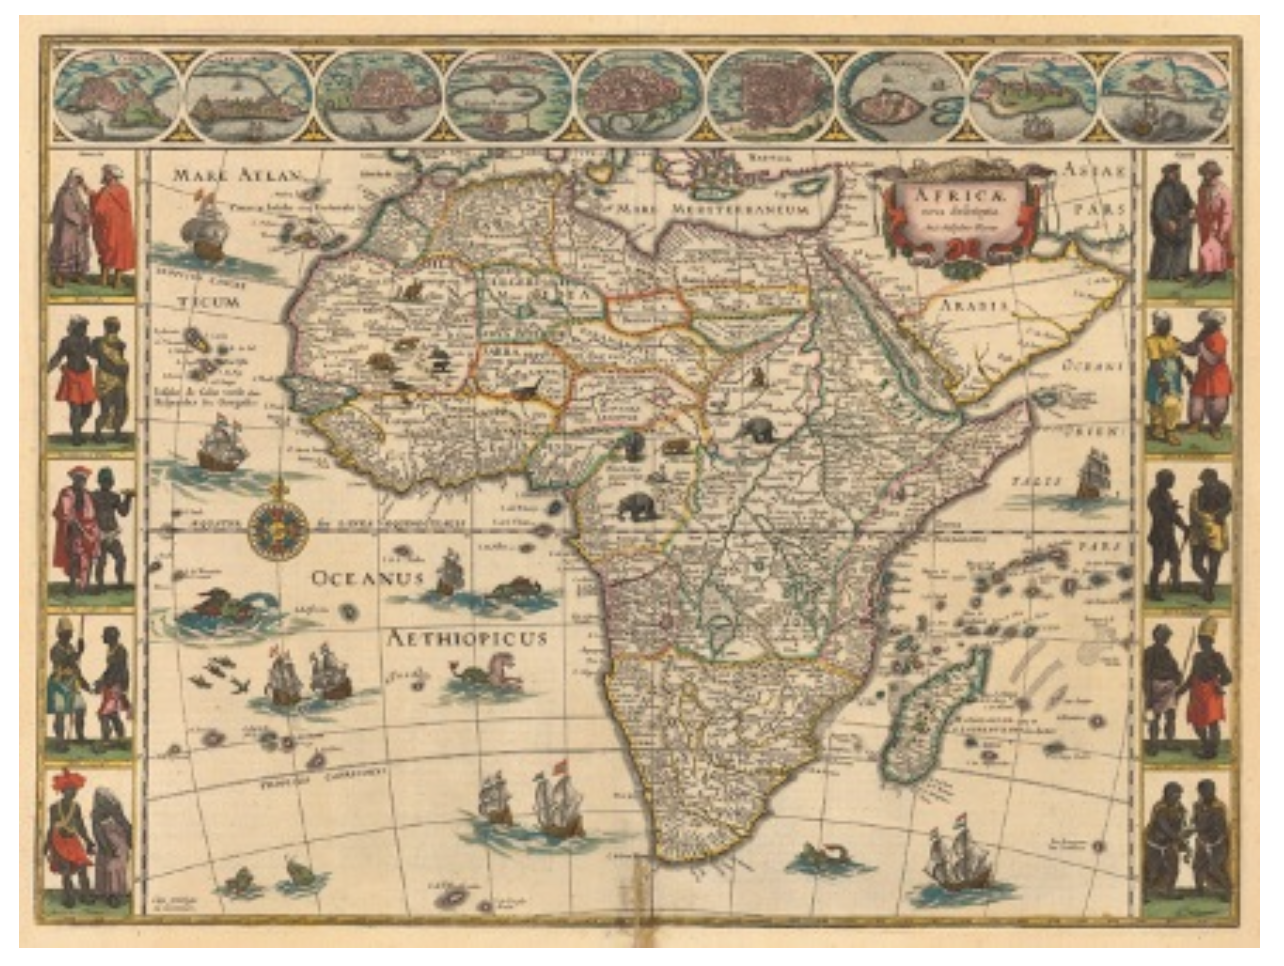
\includegraphics{./images/mapa_africa.png}

}

\caption{Origen de la Estadística}

\end{figure}

\hypertarget{estaduxedstica-vs-estaduxedstica-espacial}{%
\section{Estadística vs Estadística
Espacial}\label{estaduxedstica-vs-estaduxedstica-espacial}}

\textbf{Estadística:}

\begin{itemize}
\tightlist
\item
  Análisis de la estructura de datos representativos de una población
  (en áreas arbitrarias)
\item
  Se basa en matemáticas relativamente complejas
\end{itemize}

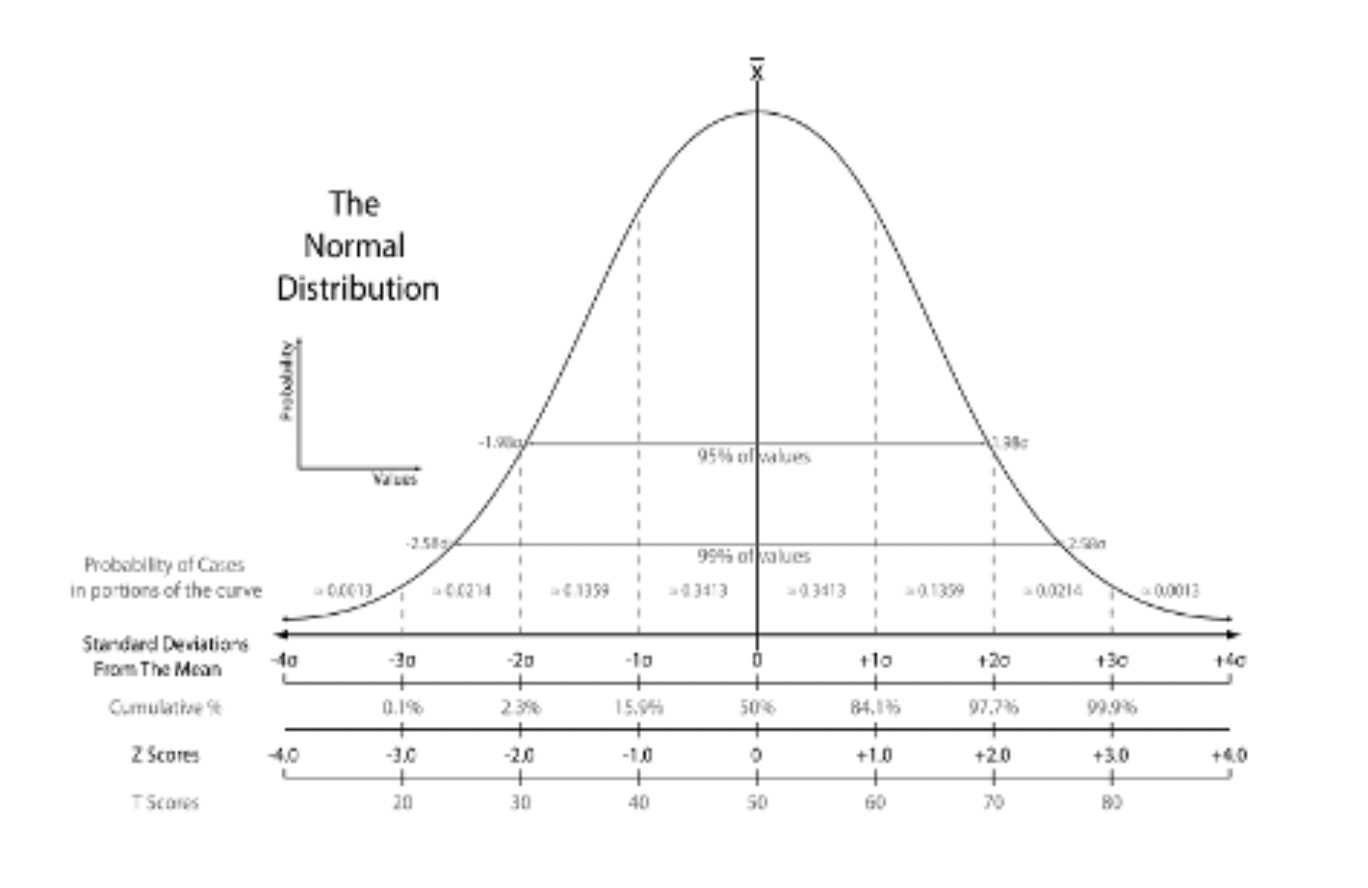
\includegraphics{./images/gauss_graph.png} \textbf{Geoestadística}

\begin{itemize}
\tightlist
\item
  Análisis de relaciones de dependencia espacial entre datos
  georreferenciados
\item
  Complejidad de cálculo que hacía inviable su uso masivo
\end{itemize}

\begin{figure}

{\centering 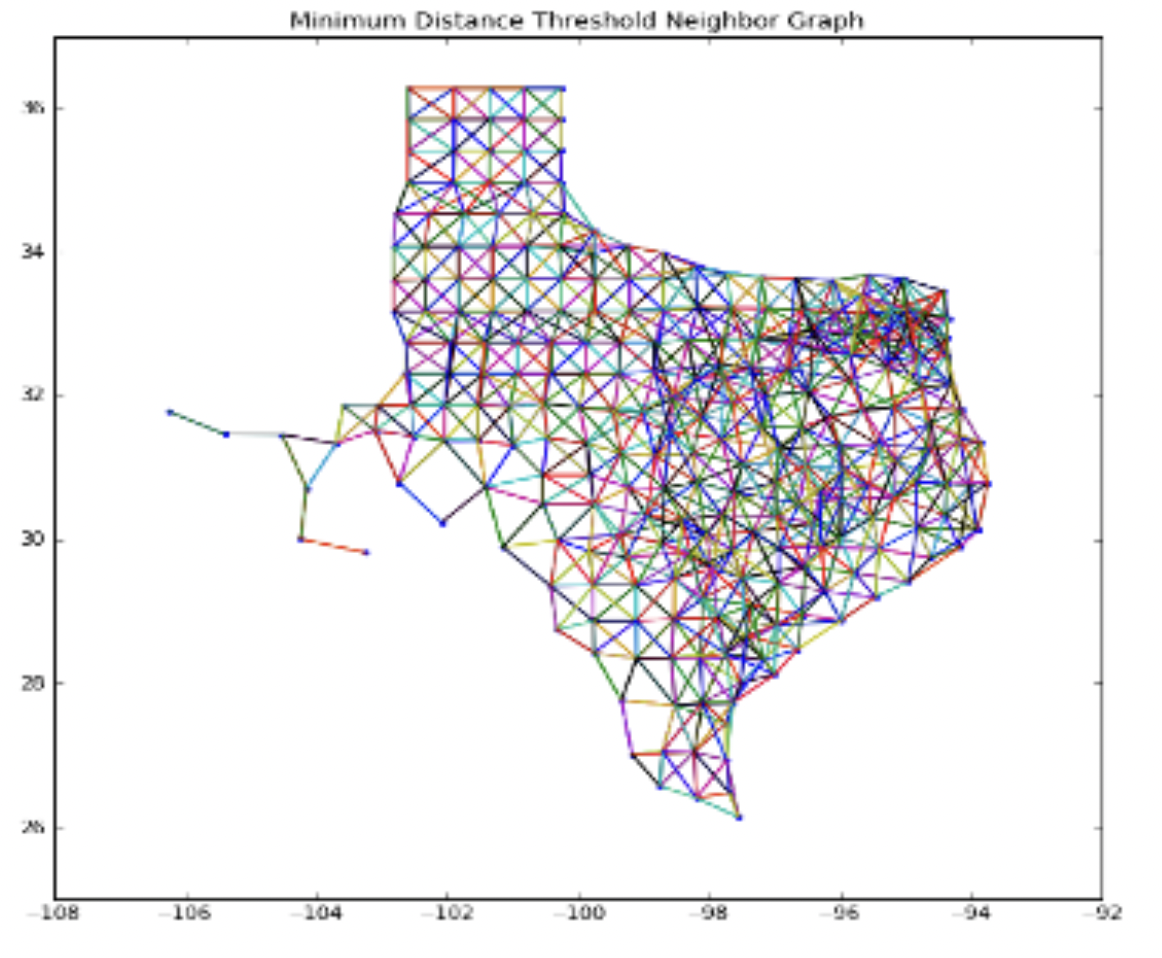
\includegraphics{./images/dep_espacial.png}

}

\caption{Dependencia espacial en geoestadística}

\end{figure}

\hypertarget{condideraciones-generales}{%
\section{Condideraciones generales}\label{condideraciones-generales}}

La inferencia estadística convencional se basa en dos supuestos
fundamentales

\begin{itemize}
\tightlist
\item
  Los valores de una variable se distribuyen de forma aleatoria
\item
  Los valores de una variable son independientes unos de otros
\end{itemize}

Pero ninguno de estos dos supuestos se cumple al utilizar datos
espaciales, ya que:

\begin{itemize}
\tightlist
\item
  Los fenómenos más próximos en el espacio están más estrechamente
  relacionados entre sí (Ley de Tobler, 1970) *La historia, el espacio y
  la sociedad se co-producen, por lo que el espacio tiene un rol activo
  en la reproducción y acumulación de fenómenos sociales (Lefebvre,
  1974)
\end{itemize}

Para resolver esta limitación existen dos enfoques principales

\begin{itemize}
\tightlist
\item
  La econometría espacial, que trata el efecto espacial como un error y
  lo elimina para generar estimaciones sin sesgo
\item
  La geoestadística, que identifica y cuantifica el efecto que el
  espacio genera en la estructura de la información
\end{itemize}

\hypertarget{ejemplos-de-correlaciuxf3n-espacial}{%
\section{Ejemplos de Correlación
Espacial}\label{ejemplos-de-correlaciuxf3n-espacial}}

\hypertarget{autoproducciuxf3n-truxe1fico-de-drogas}{%
\subsection{Autoproducción: Tráfico de
Drogas}\label{autoproducciuxf3n-truxe1fico-de-drogas}}

\begin{figure}

{\centering 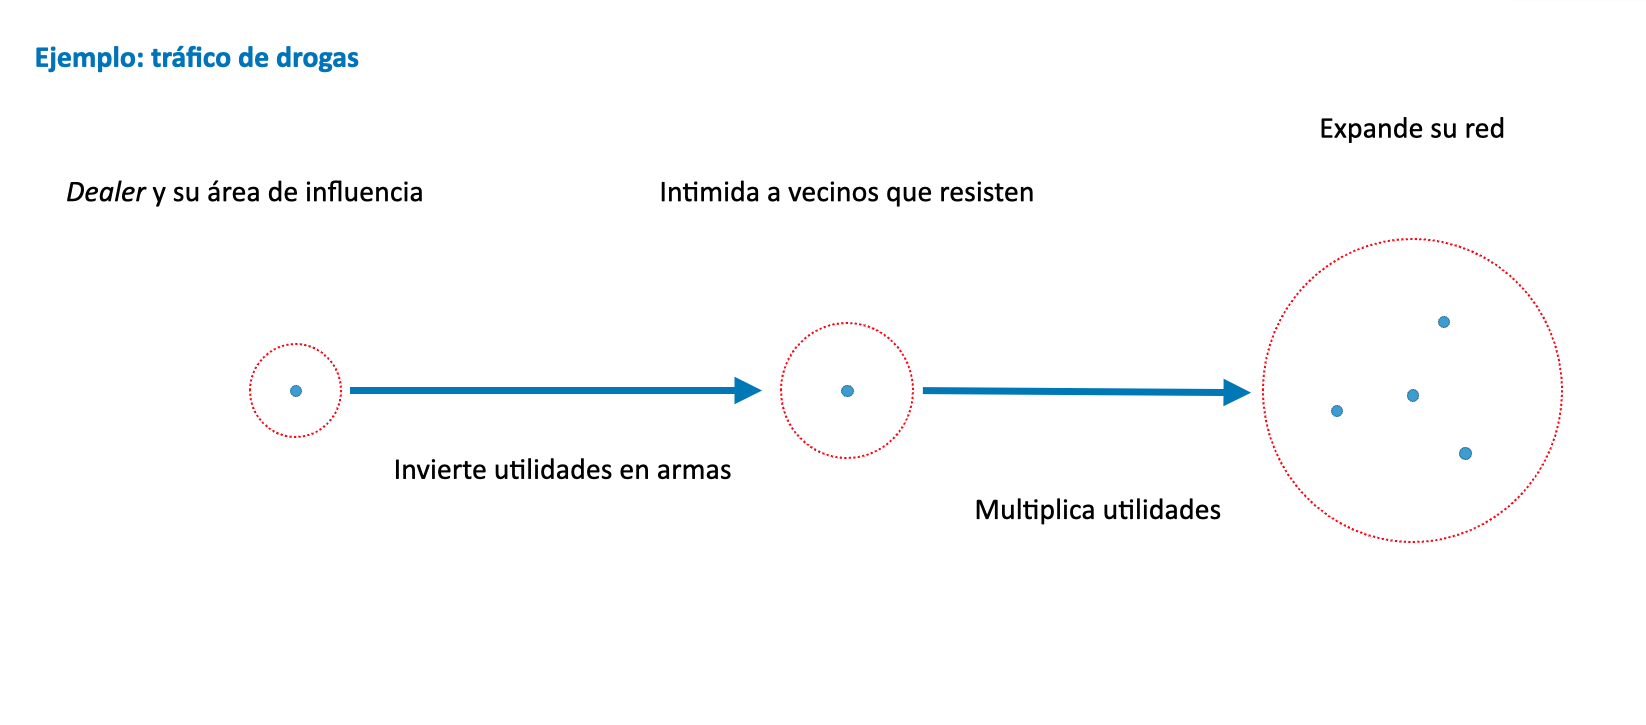
\includegraphics{./images/drogas_autoproducion.png}

}

\caption{Autoproducción Espacial en tráfico de Drogas}

\end{figure}

\hypertarget{co-producciuxf3n-mercado-inmobiliario-local}{%
\subsection{Co-producción: Mercado inmobiliario
local}\label{co-producciuxf3n-mercado-inmobiliario-local}}

\begin{figure}

{\centering 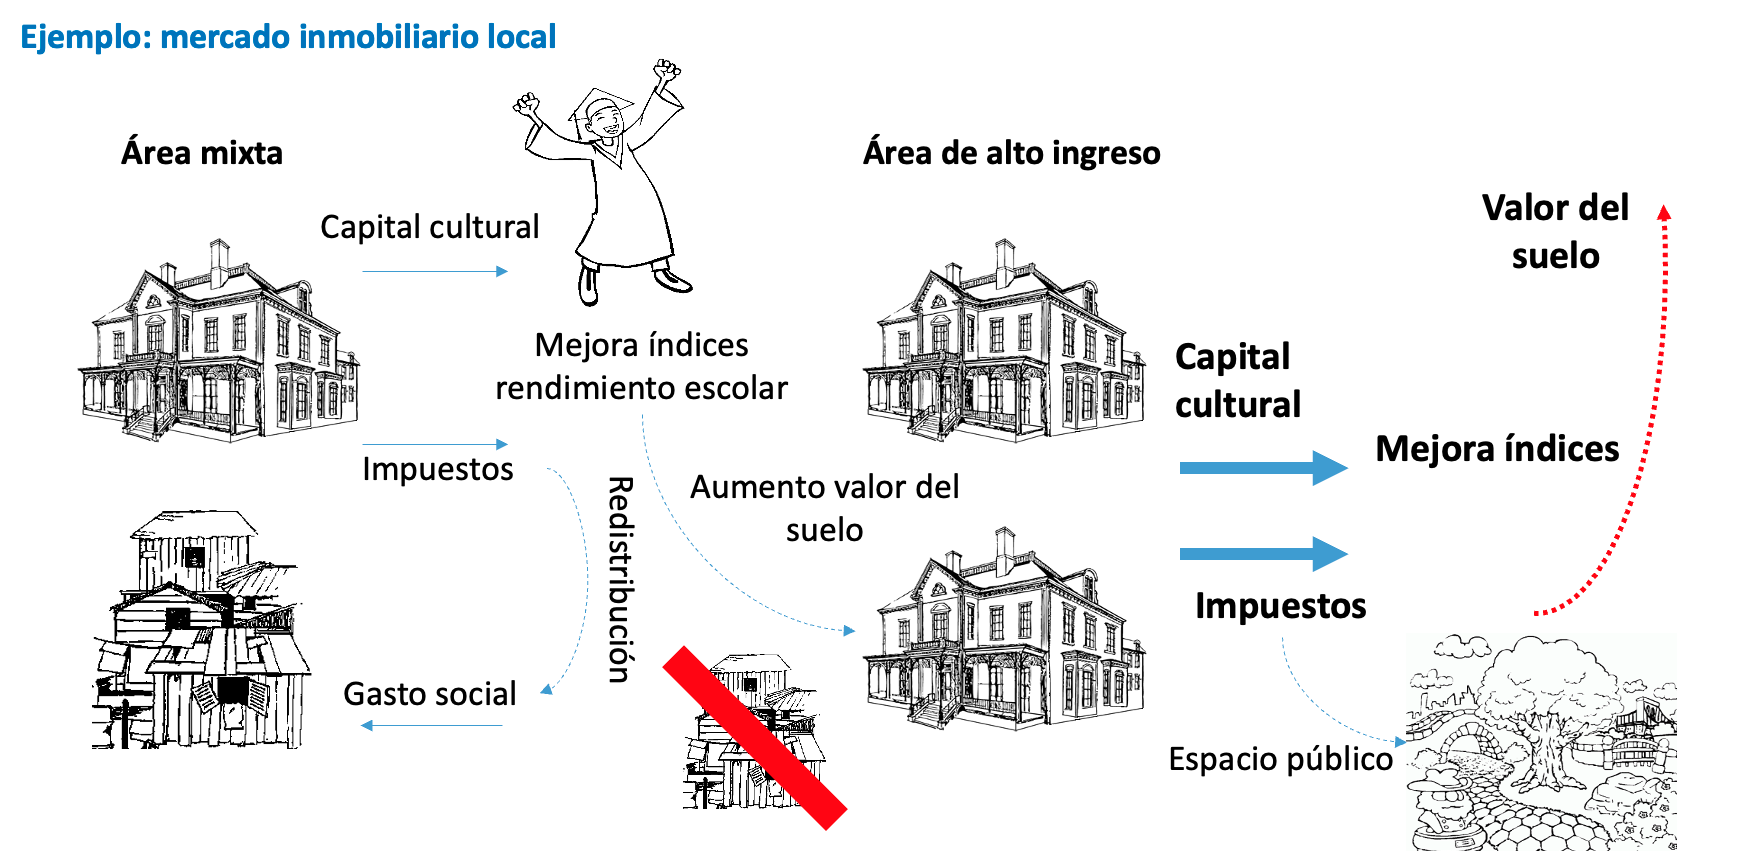
\includegraphics{./images/mercado_inmob.png}

}

\caption{Co-producción Espacial en Mercado inmobiliario local}

\end{figure}

\hypertarget{segregaciuxf3n-y-delincuencia}{%
\subsection{Segregación y
delincuencia}\label{segregaciuxf3n-y-delincuencia}}

\begin{figure}

\begin{minipage}[t]{0.33\linewidth}

{\centering 

\raisebox{-\height}{

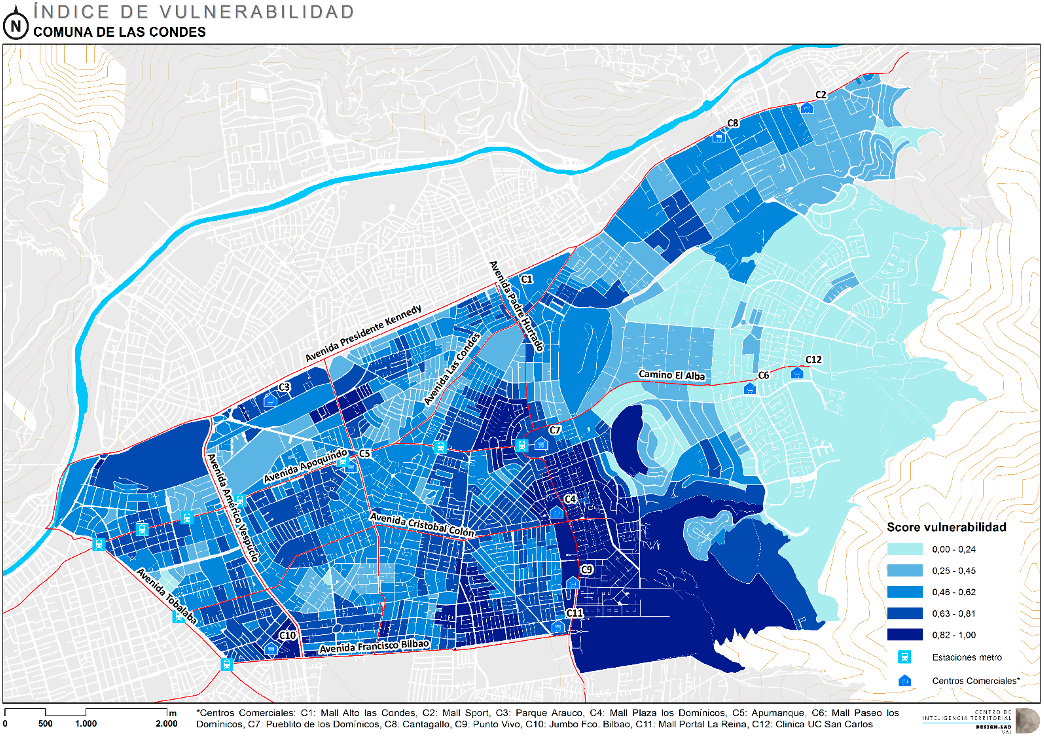
\includegraphics{./images/lc_vulnerabilidad.png}

}

}

\end{minipage}%
%
\begin{minipage}[t]{0.33\linewidth}

{\centering 

\raisebox{-\height}{

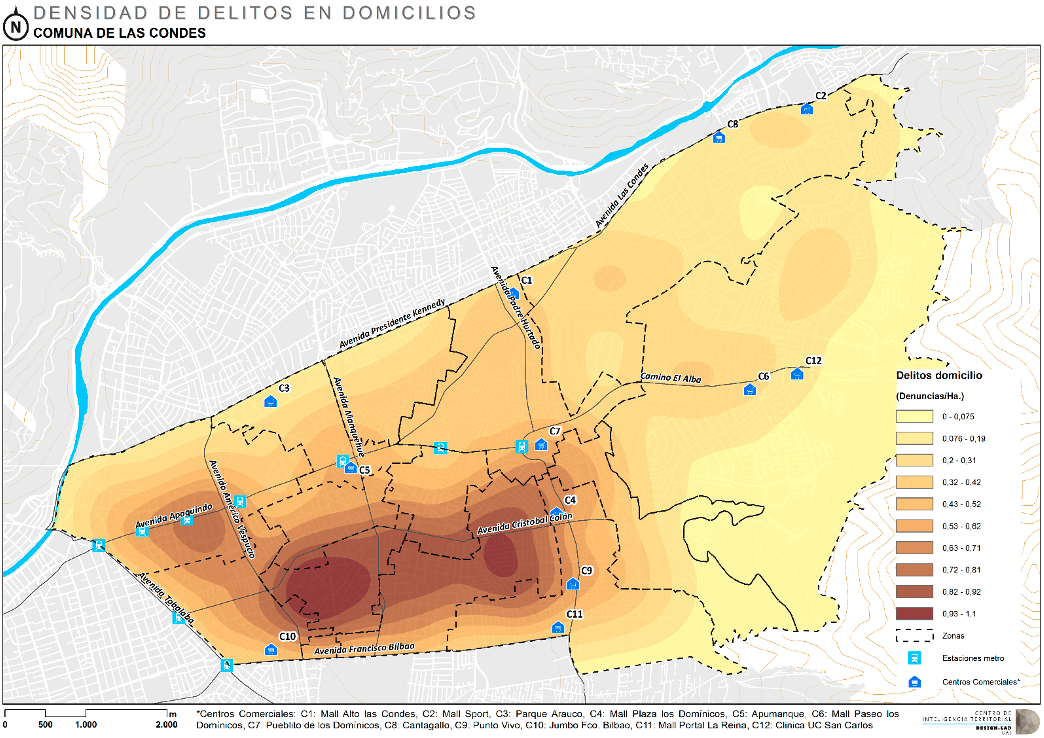
\includegraphics{./images/lc_delitos_dom.png}

}

}

\end{minipage}%
%
\begin{minipage}[t]{0.33\linewidth}

{\centering 

\raisebox{-\height}{

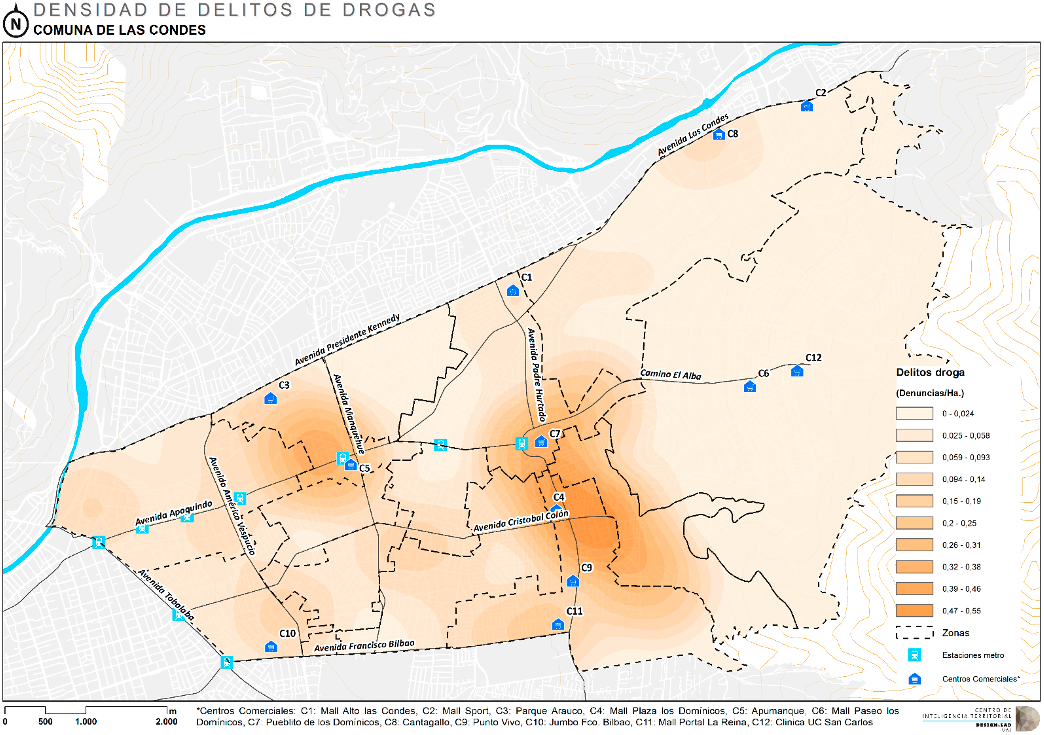
\includegraphics{./images/LC_delitos_drogas.png}

}

}

\end{minipage}%

\end{figure}

\begin{figure}

{\centering 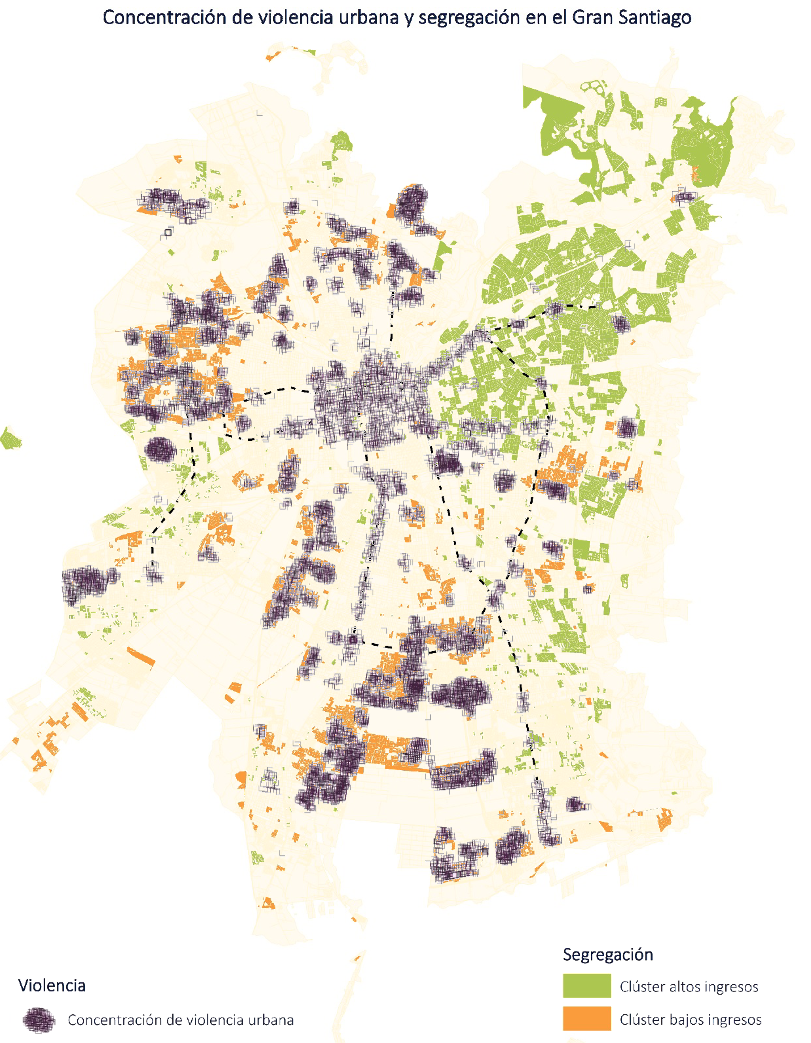
\includegraphics[width=0.7\textwidth,height=\textheight]{./images/segregacion_del.png}

}

\caption{Segregación y delincuencia}

\end{figure}

\hypertarget{valores-de-vivienda}{%
\subsection{Valores de Vivienda}\label{valores-de-vivienda}}

\begin{figure}

{\centering 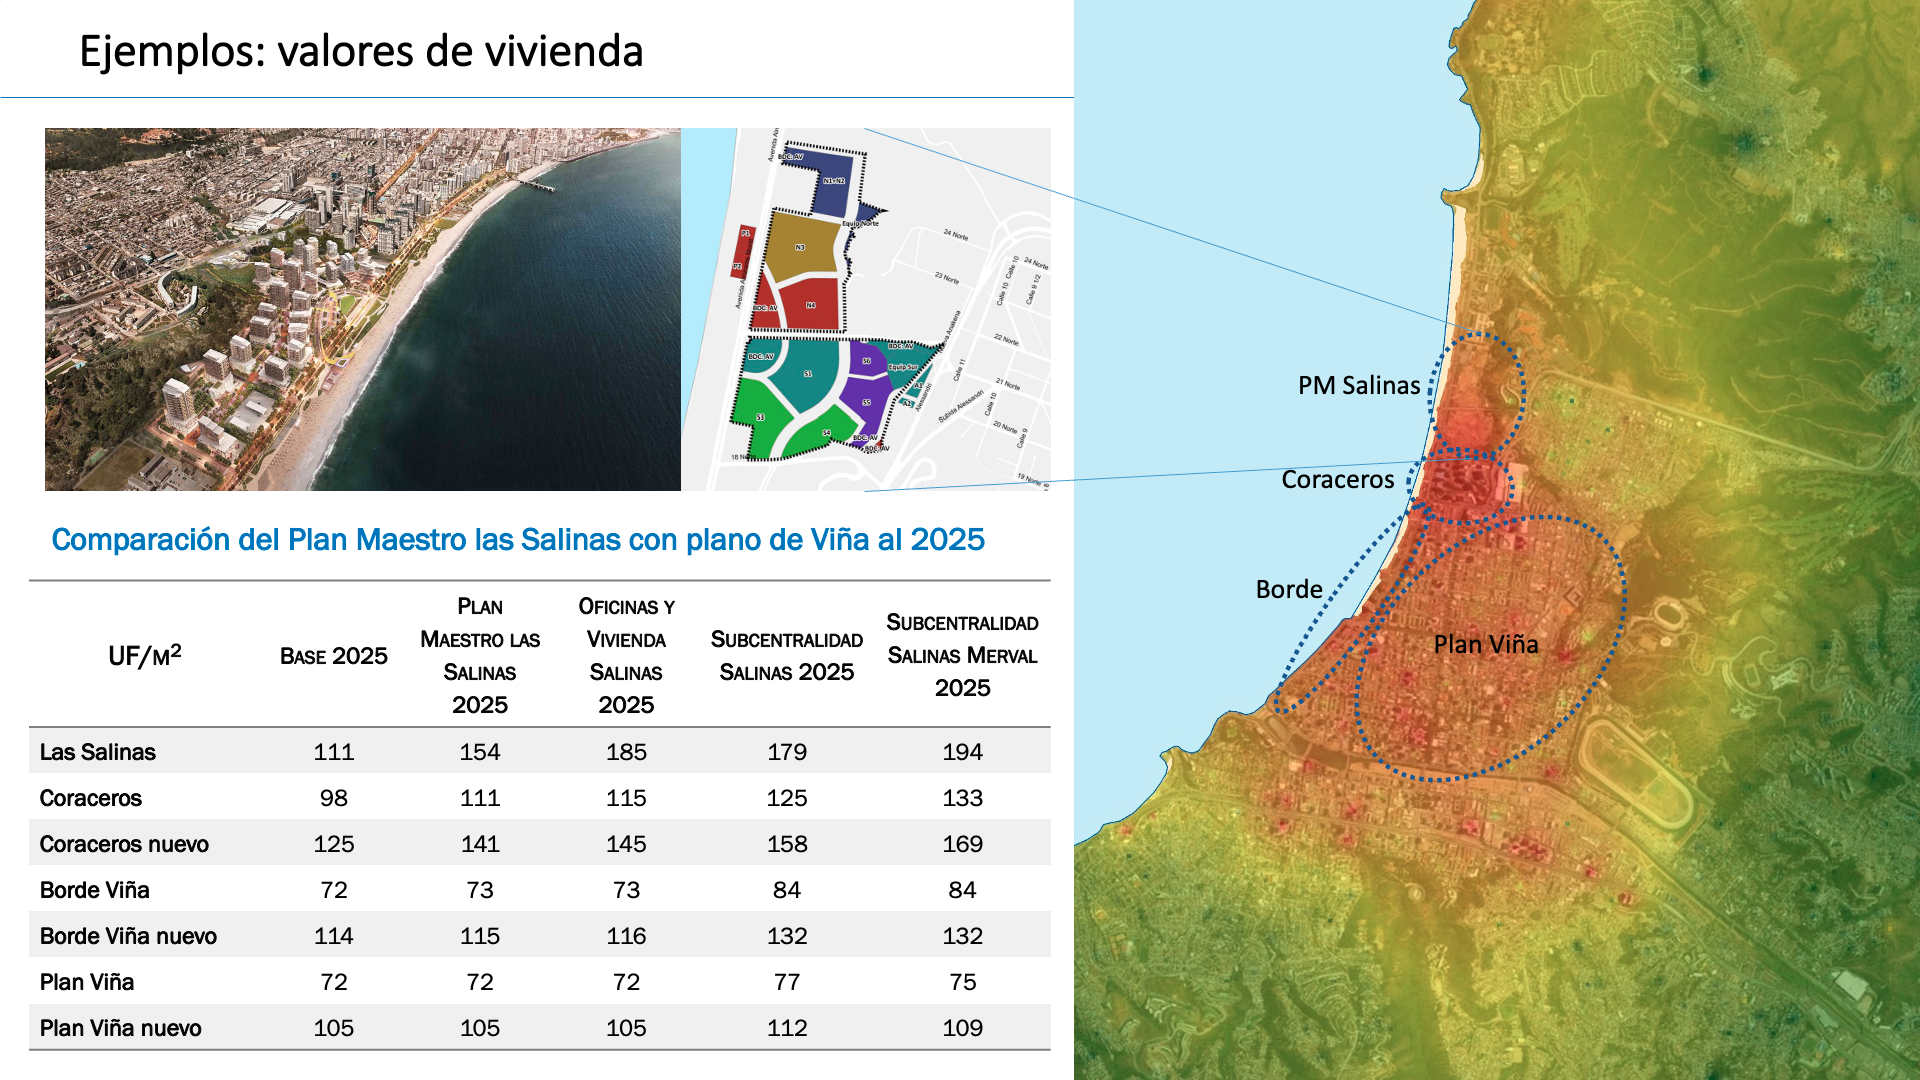
\includegraphics{./images/val_vivienda.png}

}

\caption{Valores de Vivienda}

\end{figure}

\hypertarget{inconsistencia-estaduxedstica-de-datos-espaciales-agregados-maup}{%
\section{Inconsistencia estadística de datos espaciales agregados:
MAUP}\label{inconsistencia-estaduxedstica-de-datos-espaciales-agregados-maup}}

\textbf{Modifiable Areal Unit Problem}: inconsistencia de indicadores
estadísticos al modificar los perímetros de agregación (Gehlke \& Biehl
1934, Openshaw \& Taylor 1979)

\begin{figure}

{\centering 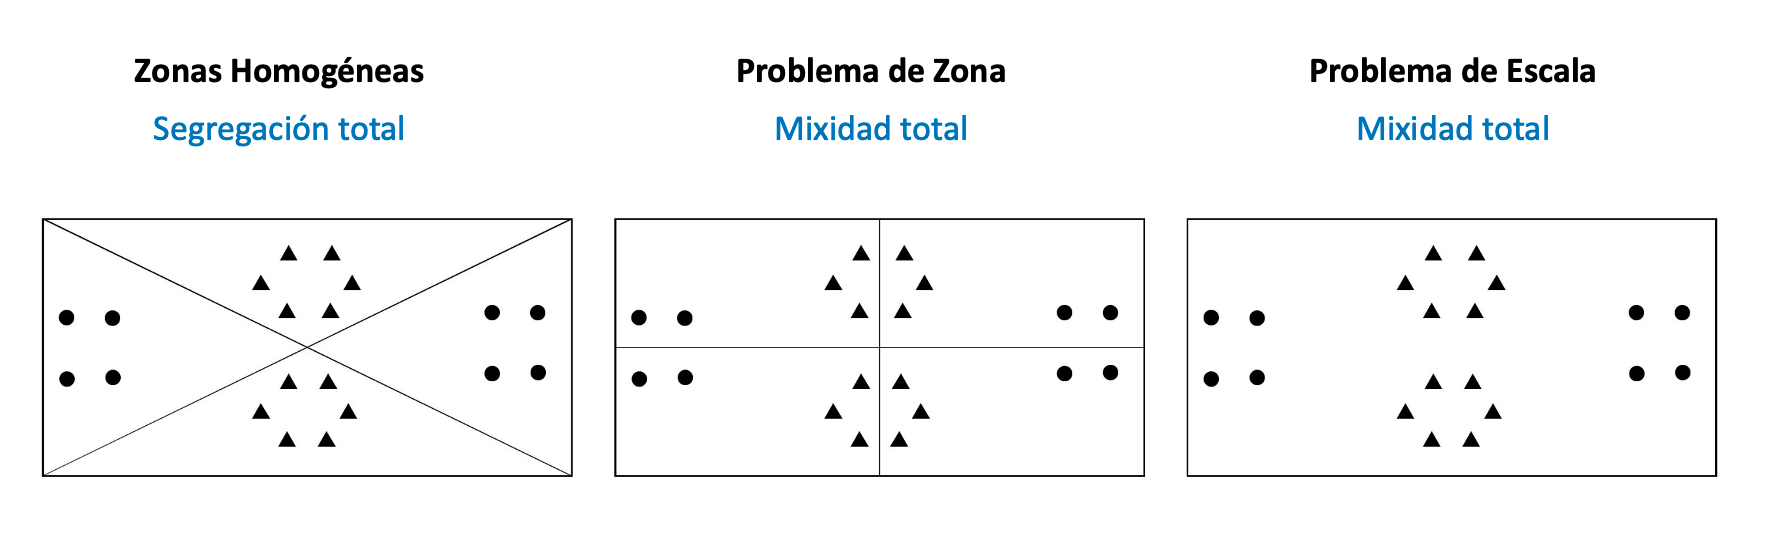
\includegraphics{./images/maup.png}

}

\caption{Modifiable Areal Unit Problem}

\end{figure}

En general, es recomendable trabajar con datos a la menor escala
posible, o agregarlos en zonas homogéneas

\bookmarksetup{startatroot}

\hypertarget{introducciuxf3n-a-datos-espaciales}{%
\chapter{Introducción a Datos
Espaciales}\label{introducciuxf3n-a-datos-espaciales}}

Módulo 1: Práctico

\hfill\break

La presente Sesión tiene como objetivo principal introducir conceptos
generales y manipulación básica de datos de tipo vectorial (punto,
lineas, polígonos) y Raster, ambos con casos prácticos.

\hypertarget{definiciuxf3n-general-de-datos-espaciales}{%
\section{Definición General de Datos
Espaciales}\label{definiciuxf3n-general-de-datos-espaciales}}

La representación de un territorio requiere datos geográficos compuestos
por información espacial (geometrías asociadas a una ubicación real en
el mundo) e información de atributos (características y variables
asociadas a estas geometrías). Los tipos de datos espaciales
principalmente los vectores y raster.

\begin{figure}

{\centering 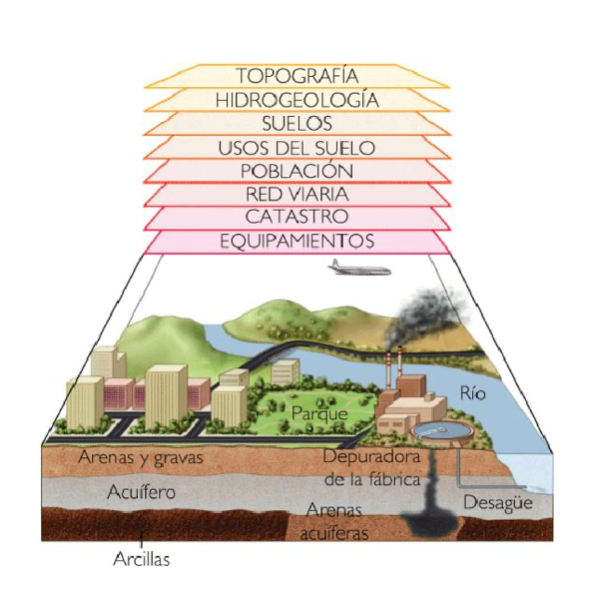
\includegraphics[width=0.5\textwidth,height=\textheight]{./images/capas_general.png}

}

\caption{Capas de datos espaciales}

\end{figure}

\hypertarget{datos-vectoriales}{%
\section{Datos Vectoriales}\label{datos-vectoriales}}

\begin{description}
\tightlist
\item[Datos Vectoriales]
Representación mediante coordenadas que se pueden unir espacialmente o
no. Corresponde a 3 tipos de geometrías: puntos, líneas y polígonos.
\end{description}

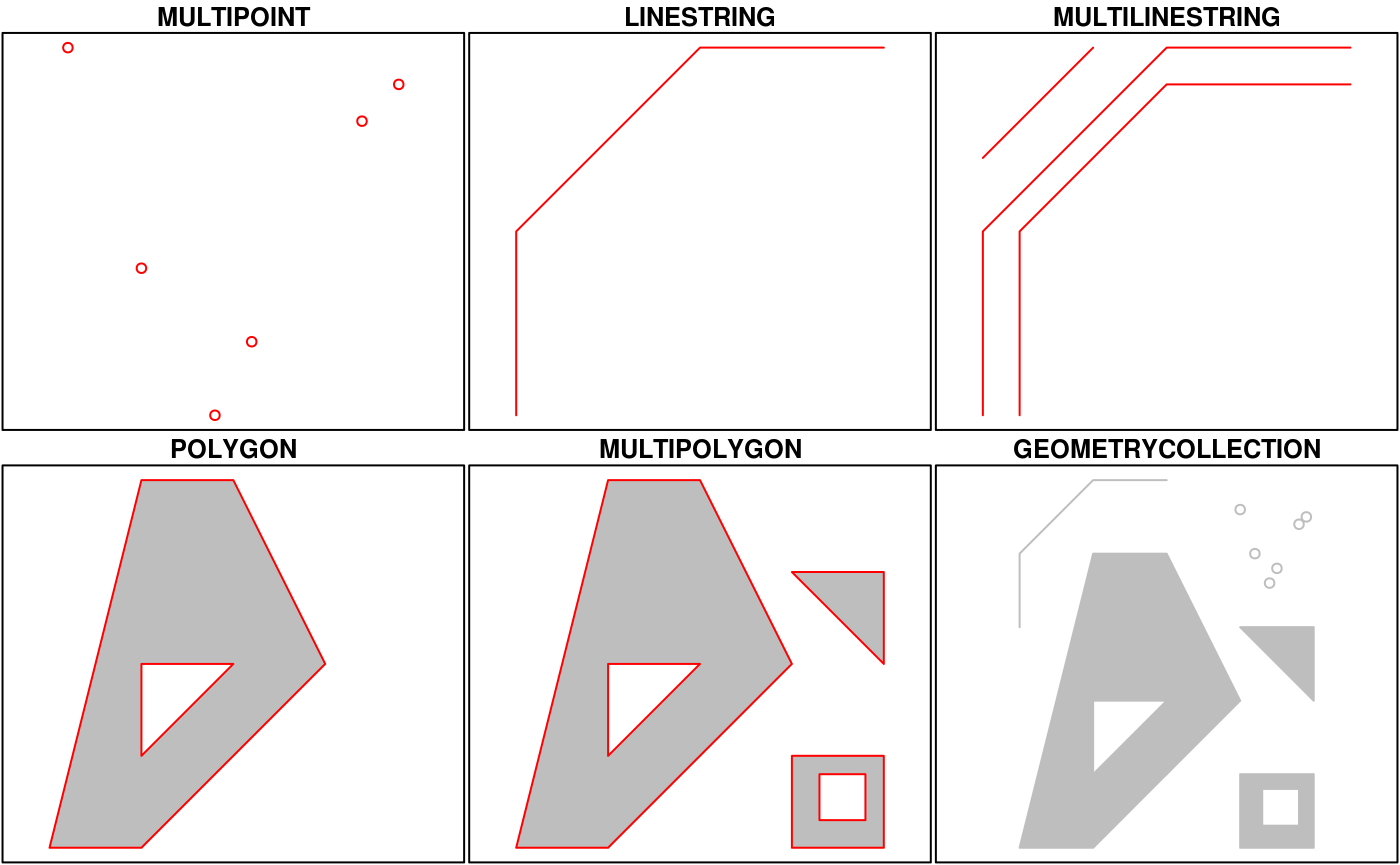
\includegraphics{./images/tipos_vect.png}

Fuente: \url{https://r-spatial.github.io/sf/articles/sf1.html}

\begin{description}
\tightlist
\item[Puntos]
Tiene un par de coordenadas ``x'' e ``y''. Es utilizado para información
de tipo puntual, como por ejemplo equipamiento urbano, postes, árboles,
entre otros.
\end{description}

\begin{figure}

{\centering 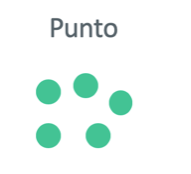
\includegraphics{./images/punto.png}

}

\caption{Objeto vectorial tipo punto}

\end{figure}

Cargar librerías

\begin{Shaded}
\begin{Highlighting}[]
\CommentTok{\# install.packages("sf") }
\FunctionTok{library}\NormalTok{(sf) }\CommentTok{\# manipulación de datos vectoriales}
\FunctionTok{library}\NormalTok{(mapview) }\CommentTok{\# visualización de mapas dinámicos}
\FunctionTok{library}\NormalTok{(ggplot2) }\CommentTok{\# gráficos}
\FunctionTok{library}\NormalTok{(RColorBrewer) }\CommentTok{\#paleta de colores}
\end{Highlighting}
\end{Shaded}

\hypertarget{lectura-de-archivos-tipo-puntos}{%
\subsection{Lectura de archivos tipo
puntos}\label{lectura-de-archivos-tipo-puntos}}

\begin{Shaded}
\begin{Highlighting}[]
\NormalTok{sii\_LC }\OtherTok{\textless{}{-}} \FunctionTok{st\_read}\NormalTok{(}\StringTok{"data/sii/sii\_urbe\_LC.shp"}\NormalTok{)}
\end{Highlighting}
\end{Shaded}

\begin{verbatim}
Reading layer `sii_urbe_LC' from data source 
  `/Users/denisberroeta/Library/CloudStorage/OneDrive-UniversidadAdolfoIbanez/Goblab/BDPP_2022/geoanalisis_book/data/sii/sii_urbe_LC.shp' 
  using driver `ESRI Shapefile'
Simple feature collection with 2310 features and 11 fields
Geometry type: POINT
Dimension:     XY
Bounding box:  xmin: -70.60645 ymin: -33.44471 xmax: -70.47083 ymax: -33.36548
Geodetic CRS:  GCS_unknown
\end{verbatim}

\hypertarget{visualizaciuxf3n-de-los-puntos}{%
\subsection{Visualización de los
puntos}\label{visualizaciuxf3n-de-los-puntos}}

\begin{Shaded}
\begin{Highlighting}[]
\CommentTok{\# Visualización ggplot y sf}
\FunctionTok{ggplot}\NormalTok{() }\SpecialCharTok{+}
  \FunctionTok{geom\_sf}\NormalTok{(}\AttributeTok{data =}\NormalTok{ sii\_LC, }\AttributeTok{col =} \StringTok{"orange"}\NormalTok{, }\AttributeTok{alpha=}\FloatTok{0.8}\NormalTok{,  }\AttributeTok{size=} \FloatTok{0.5}\NormalTok{)}\SpecialCharTok{+}
  \FunctionTok{ggtitle}\NormalTok{(}\StringTok{"Datos del SII en Las Condes"}\NormalTok{ ) }\SpecialCharTok{+}
  \FunctionTok{theme\_bw}\NormalTok{() }\SpecialCharTok{+}
  \FunctionTok{theme}\NormalTok{(}\AttributeTok{legend.position=}\StringTok{"none"}\NormalTok{)}\SpecialCharTok{+}
  \FunctionTok{theme}\NormalTok{(}\AttributeTok{panel.grid.major =} \FunctionTok{element\_line}\NormalTok{(}\AttributeTok{colour =} \StringTok{"gray80"}\NormalTok{), }
        \AttributeTok{panel.grid.minor =} \FunctionTok{element\_line}\NormalTok{(}\AttributeTok{colour =} \StringTok{"gray80"}\NormalTok{))}
\end{Highlighting}
\end{Shaded}

\begin{figure}[H]

{\centering 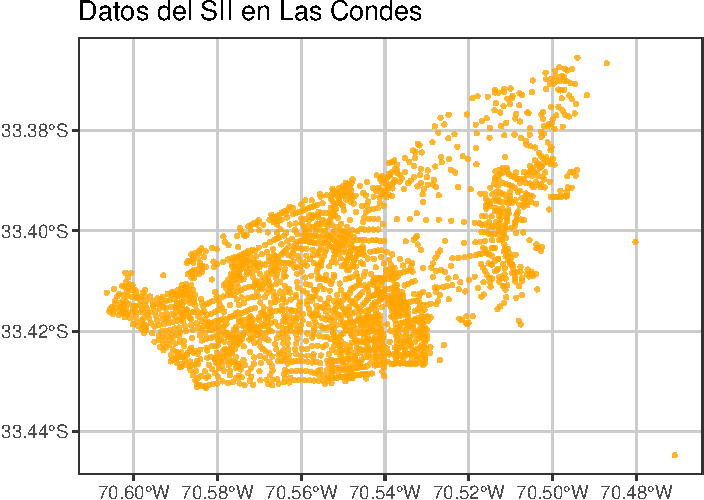
\includegraphics{./datos_espaciales_files/figure-pdf/unnamed-chunk-3-1.pdf}

}

\end{figure}

\begin{Shaded}
\begin{Highlighting}[]
\CommentTok{\# mapview(sii\_LC, zcol = "atractor", cex =2)}
\end{Highlighting}
\end{Shaded}

\begin{description}
\tightlist
\item[Líneas]
Tiene tantas coordenadas como vértices. La información que representa es
de tipo lineal, como por ejemplo calles, ríos, redes energéticas, entre
otros. Existen las líneas cerradas, las cuales se pueden entender como
el perímetro de una superficie (sin relleno).
\end{description}

\begin{figure}

{\centering 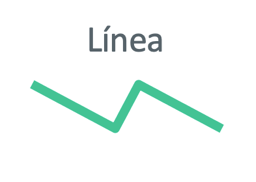
\includegraphics{./images/linea.png}

}

\caption{Objeto vectorial tipo Línea}

\end{figure}

\hypertarget{lectura-de-luxedneas}{%
\subsection{Lectura de líneas}\label{lectura-de-luxedneas}}

\begin{Shaded}
\begin{Highlighting}[]
\NormalTok{las\_condes\_red }\OtherTok{\textless{}{-}} \FunctionTok{readRDS}\NormalTok{(}\StringTok{"data/redes/RED\_LAS\_CONDES.rds"}\NormalTok{) }
\CommentTok{\# las\_condes\_red}
\end{Highlighting}
\end{Shaded}

\hypertarget{visualizaciuxf3n-luxedneas}{%
\subsection{visualización Líneas}\label{visualizaciuxf3n-luxedneas}}

\begin{Shaded}
\begin{Highlighting}[]
\FunctionTok{ggplot}\NormalTok{() }\SpecialCharTok{+}
  \FunctionTok{geom\_sf}\NormalTok{(}\AttributeTok{data =}\NormalTok{ las\_condes\_red, }\AttributeTok{col =} \StringTok{"gray70"}\NormalTok{, }\AttributeTok{alpha=}\FloatTok{0.8}\NormalTok{,  }\AttributeTok{size=} \FloatTok{0.5}\NormalTok{)}\SpecialCharTok{+}
  \FunctionTok{ggtitle}\NormalTok{(}\StringTok{"Red víal de la comuna Las Condes"}\NormalTok{ ) }\SpecialCharTok{+}
  \FunctionTok{theme\_bw}\NormalTok{() }\SpecialCharTok{+}
  \FunctionTok{theme}\NormalTok{(}\AttributeTok{legend.position=}\StringTok{"none"}\NormalTok{)}\SpecialCharTok{+}
  \FunctionTok{theme}\NormalTok{(}\AttributeTok{panel.grid.major =} \FunctionTok{element\_line}\NormalTok{(}\AttributeTok{colour =} \StringTok{"gray80"}\NormalTok{), }
        \AttributeTok{panel.grid.minor =} \FunctionTok{element\_line}\NormalTok{(}\AttributeTok{colour =} \StringTok{"gray80"}\NormalTok{))}
\end{Highlighting}
\end{Shaded}

\begin{figure}[H]

{\centering 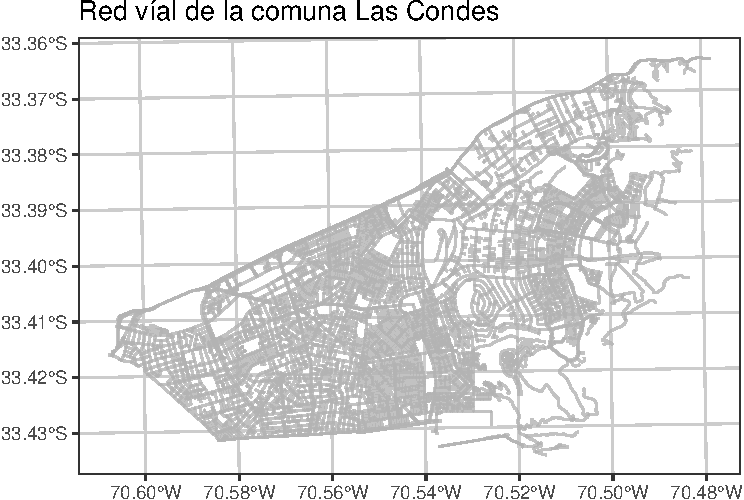
\includegraphics{./datos_espaciales_files/figure-pdf/unnamed-chunk-5-1.pdf}

}

\end{figure}

\begin{Shaded}
\begin{Highlighting}[]
\CommentTok{\# mapview(las\_condes\_red)}
\end{Highlighting}
\end{Shaded}

\begin{description}
\tightlist
\item[Polígonos]
Tiene tantas coordenadas como vértices. La información que representa es
de tipo área, como por ejemplo división política administrativa,
manzanas, construcciones, entre otras.
\end{description}

\begin{figure}

{\centering 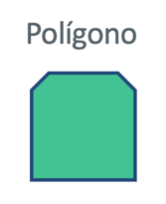
\includegraphics{./images/poligono.png}

}

\caption{Objeto vectorial tipo polígono}

\end{figure}

\hypertarget{lectura-de-poluxedgonos}{%
\subsection{Lectura de polígonos}\label{lectura-de-poluxedgonos}}

\begin{Shaded}
\begin{Highlighting}[]
\NormalTok{las\_condes\_mz }\OtherTok{\textless{}{-}} \FunctionTok{st\_read}\NormalTok{(}\StringTok{"data/shape/icv\_las\_condes.shp"}\NormalTok{, }\AttributeTok{quiet=}\NormalTok{T) }
\CommentTok{\# las\_condes\_ptos}
\end{Highlighting}
\end{Shaded}

\hypertarget{visualizaciuxf3n-poluxedgonos}{%
\subsection{Visualización
polígonos}\label{visualizaciuxf3n-poluxedgonos}}

\begin{Shaded}
\begin{Highlighting}[]
\FunctionTok{ggplot}\NormalTok{() }\SpecialCharTok{+}
  \FunctionTok{geom\_sf}\NormalTok{(}\AttributeTok{data =}\NormalTok{ las\_condes\_mz, }\FunctionTok{aes}\NormalTok{(}\AttributeTok{fill =}\NormalTok{ veg\_cob), }\AttributeTok{color =}\StringTok{"gray80"}\NormalTok{, }
          \AttributeTok{alpha=}\FloatTok{0.8}\NormalTok{,  }\AttributeTok{size=} \FloatTok{0.1}\NormalTok{)}\SpecialCharTok{+}
  \FunctionTok{scale\_fill\_distiller}\NormalTok{(}\AttributeTok{palette=}\StringTok{"Greens"}\NormalTok{, }\AttributeTok{direction =} \DecValTok{1}\NormalTok{)}\SpecialCharTok{+}
  \FunctionTok{ggtitle}\NormalTok{(}\StringTok{"Cobertura Vegetal de la comuna Las Condes"}\NormalTok{ ) }\SpecialCharTok{+}
  \FunctionTok{theme\_bw}\NormalTok{() }\SpecialCharTok{+}
  \FunctionTok{theme}\NormalTok{(}\AttributeTok{panel.grid.major =} \FunctionTok{element\_line}\NormalTok{(}\AttributeTok{colour =} \StringTok{"gray80"}\NormalTok{), }
        \AttributeTok{panel.grid.minor =} \FunctionTok{element\_line}\NormalTok{(}\AttributeTok{colour =} \StringTok{"gray80"}\NormalTok{))}
\end{Highlighting}
\end{Shaded}

\begin{figure}[H]

{\centering 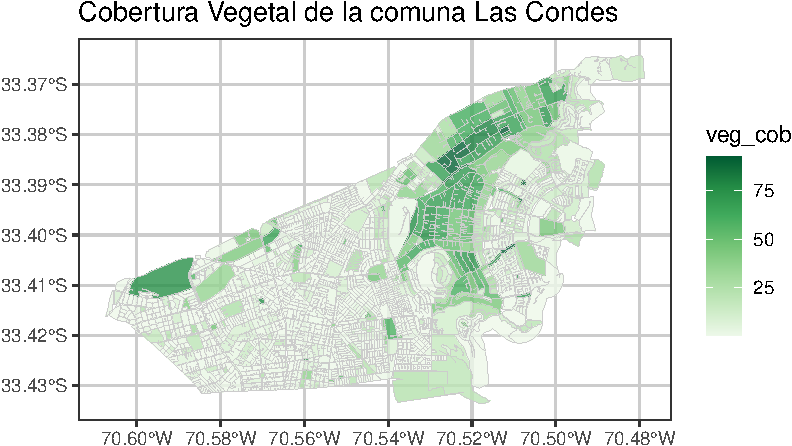
\includegraphics{./datos_espaciales_files/figure-pdf/unnamed-chunk-7-1.pdf}

}

\end{figure}

\begin{Shaded}
\begin{Highlighting}[]
\CommentTok{\# mapview(las\_condes\_mz, zcol = "veg\_cob")}
\end{Highlighting}
\end{Shaded}

\textbf{Tabla General de tipo de Datos Vectoriales}

\begin{longtable}[]{@{}
  >{\raggedright\arraybackslash}p{(\columnwidth - 2\tabcolsep) * \real{0.5000}}
  >{\raggedright\arraybackslash}p{(\columnwidth - 2\tabcolsep) * \real{0.5000}}@{}}
\toprule()
\begin{minipage}[b]{\linewidth}\raggedright
type
\end{minipage} & \begin{minipage}[b]{\linewidth}\raggedright
description
\end{minipage} \\
\midrule()
\endhead
POINT & zero-dimensional geometry containing a single point \\
LINESTRING & sequence of points connected by straight, non-self
intersecting line pieces; one-dimensional geometry \\
POLYGON & geometry with a positive area (two-dimensional); sequence of
points form a closed, non-self intersecting ring; the first ring denotes
the exterior ring, zero or more subsequent rings denote holes in this
exterior ring \\
MULTIPOINT & set of points; a MULTIPOINT is simple if no two Points in
the MULTIPOINT are equal \\
MULTILINESTRING & set of linestrings \\
MULTIPOLYGON & set of polygons \\
GEOMETRYCOLLECTION & set of geometries of any type except
GEOMETRYCOLLECTION \\
\bottomrule()
\end{longtable}

\begin{figure}

{\centering 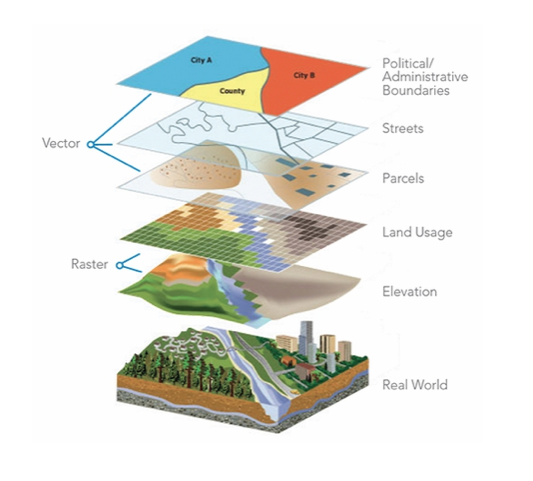
\includegraphics[width=0.7\textwidth,height=\textheight]{./images/capas.png}

}

\caption{Capas de datos tipos raster y vectores}

\end{figure}

\hypertarget{datos-raster}{%
\section{Datos Raster}\label{datos-raster}}

\begin{description}
\tightlist
\item[Raster]
Representación del espacio mediante una matriz de celdas organizada en
filas y columnas, donde cada celda tiene un valor que representa
información.
\end{description}

\begin{figure}

{\centering 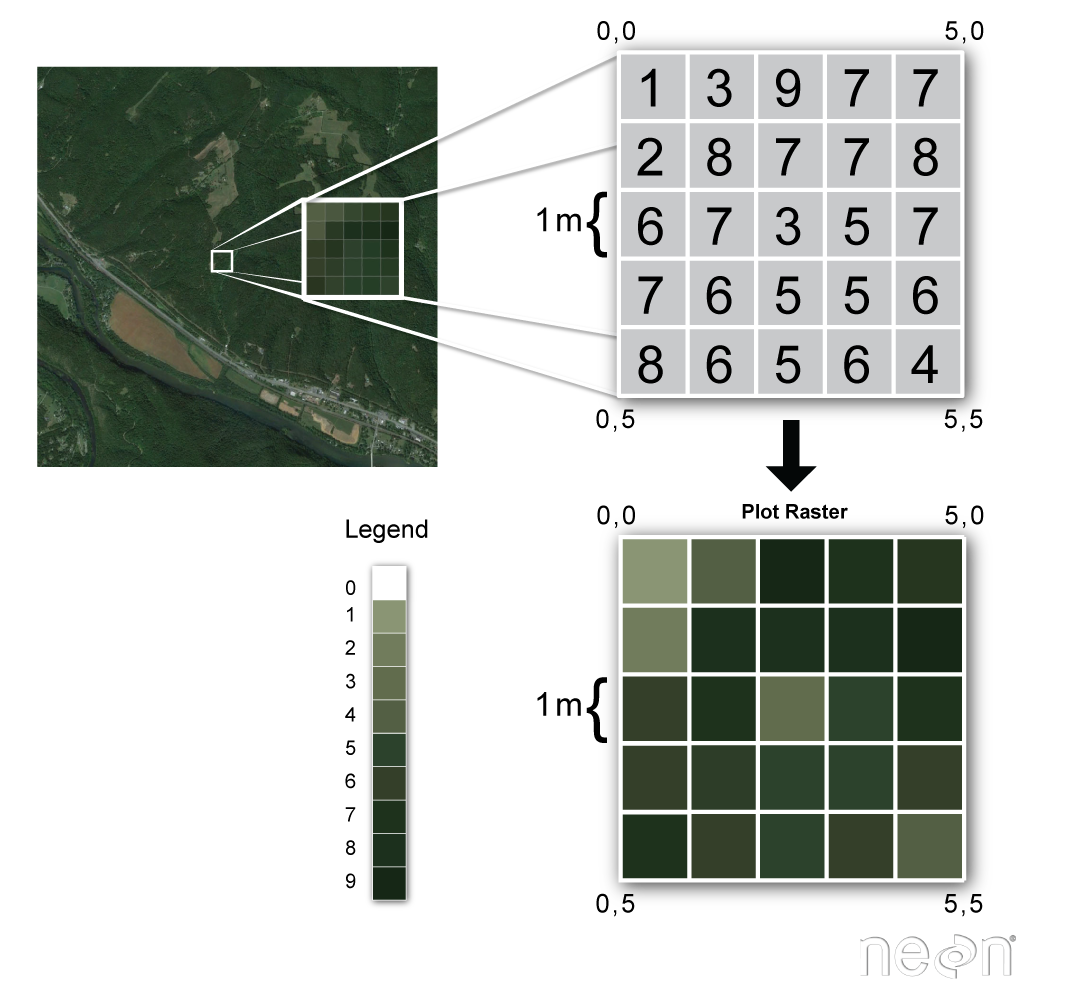
\includegraphics[width=0.6\textwidth,height=\textheight]{./images/raster_concept.png}

}

\caption{Representación Raster}

\end{figure}

\begin{figure}

{\centering \includegraphics{./images/raster_resolucion.gif}

}

\caption{Resolución Raster}

\end{figure}

Para ejemplificar el uso y ver características de Raster vamos a
utilizar una imágenes satelital del
\href{https://eos.com/es/find-satellite/landsat-8/}{Satelite Landsat 8}.

\begin{figure}

{\centering 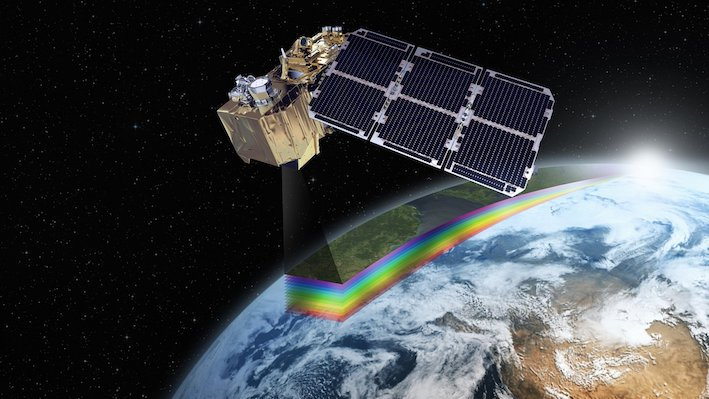
\includegraphics{./images/Sentinel-2Poster.jpg}

}

\caption{Imágenes Satelitales}

\end{figure}

Este tipos de imágenes satelitales generalmente contiene una series de
de bandas que corresponden a capas de información tipos raster
conformando una especie de brick de raster.

\begin{figure}

{\centering 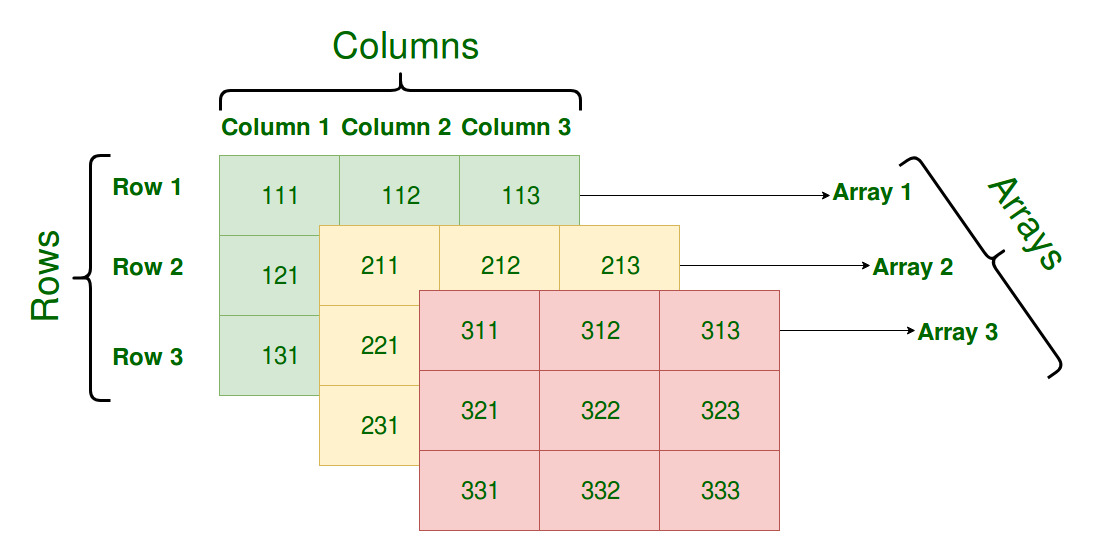
\includegraphics{./images/3D-array.jpg}

}

\caption{Configuración de Bandas}

\end{figure}

Para este ejemplo de visualización necesitamos conocer las bandas
satelitales que componen nuestra imagen satelital.

\begin{figure}

{\centering 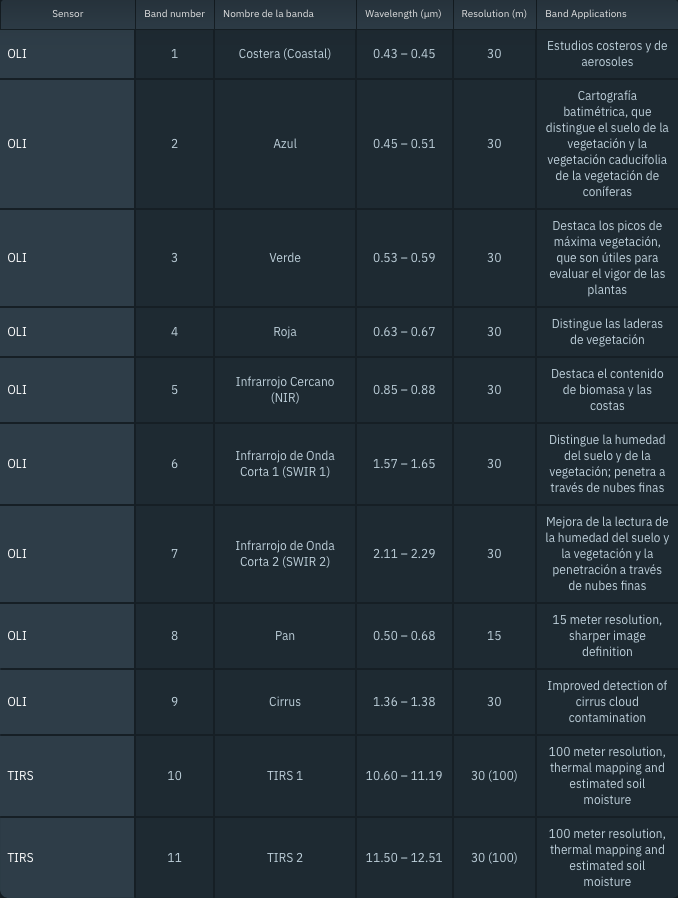
\includegraphics{./images/bandas_landsat8.png}

}

\caption{Bandas de Landsat 8}

\end{figure}

\hypertarget{lectura-de-imagen-raster.}{%
\subsection{lectura de imagen Raster.}\label{lectura-de-imagen-raster.}}

\begin{Shaded}
\begin{Highlighting}[]
\FunctionTok{library}\NormalTok{(raster)}
\NormalTok{las\_condes\_raster }\OtherTok{\textless{}{-}} \FunctionTok{brick}\NormalTok{(}\StringTok{"data/raster/OLI\_LC.tif"}\NormalTok{)}
\FunctionTok{names}\NormalTok{(las\_condes\_raster) }\OtherTok{\textless{}{-}} \FunctionTok{c}\NormalTok{(}\StringTok{"aerosol"}\NormalTok{, }\StringTok{"blue"}\NormalTok{, }\StringTok{"green"}\NormalTok{, }\StringTok{"red"}\NormalTok{ , }\StringTok{"nir"}\NormalTok{, }\StringTok{"swir1"}\NormalTok{, }\StringTok{"swir2"}\NormalTok{, }\StringTok{"tirs1"}\NormalTok{)}
\NormalTok{las\_condes\_raster}
\end{Highlighting}
\end{Shaded}

\begin{verbatim}
class      : RasterBrick 
dimensions : 449, 562, 252338, 8  (nrow, ncol, ncell, nlayers)
resolution : 30, 30  (x, y)
extent     : 350505, 367365, 6293905, 6307375  (xmin, xmax, ymin, ymax)
crs        : +proj=utm +zone=19 +south +datum=WGS84 +units=m +no_defs 
source     : OLI_LC.tif 
names      : aerosol,  blue, green,   red,   nir, swir1, swir2, tirs1 
min values :    8465,  7604,  6500,  5924,  5520,  5191,  5197,  5002 
max values :   19119, 20517, 21248, 23237, 29344, 30012, 31166,  5512 
\end{verbatim}

\hypertarget{visualizaciuxf3n-raster}{%
\subsection{Visualización Raster}\label{visualizaciuxf3n-raster}}

\begin{Shaded}
\begin{Highlighting}[]
\CommentTok{\# Visualización de imagen recortada de Las Condes en Color Natural}
\FunctionTok{plotRGB}\NormalTok{(las\_condes\_raster, }\AttributeTok{r =} \DecValTok{4}\NormalTok{, }\AttributeTok{g =} \DecValTok{3}\NormalTok{, }\AttributeTok{b =} \DecValTok{2}\NormalTok{, }\AttributeTok{stretch =} \StringTok{"lin"}\NormalTok{)}
\end{Highlighting}
\end{Shaded}

\begin{figure}[H]

{\centering 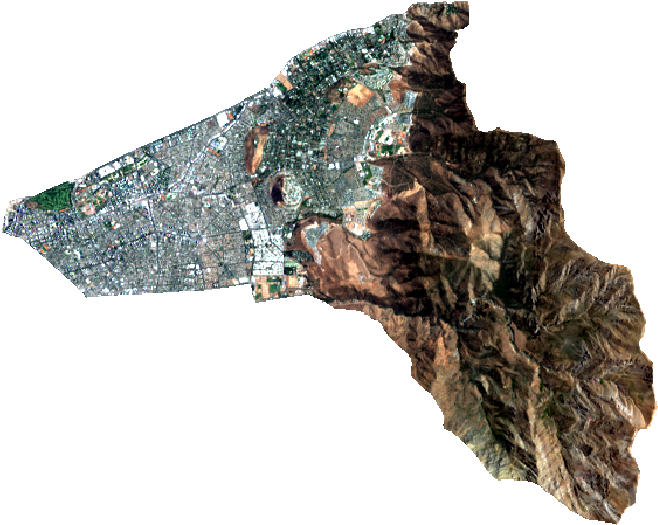
\includegraphics{./datos_espaciales_files/figure-pdf/unnamed-chunk-9-1.pdf}

}

\end{figure}

\begin{Shaded}
\begin{Highlighting}[]
\CommentTok{\# viewRGB(las\_condes\_raster, r = 4, g = 3, b = 2)}
\end{Highlighting}
\end{Shaded}

\hypertarget{sistema-de-referencias-de-coordenadas}{%
\section{Sistema de Referencias de
Coordenadas}\label{sistema-de-referencias-de-coordenadas}}

\begin{figure}

{\centering 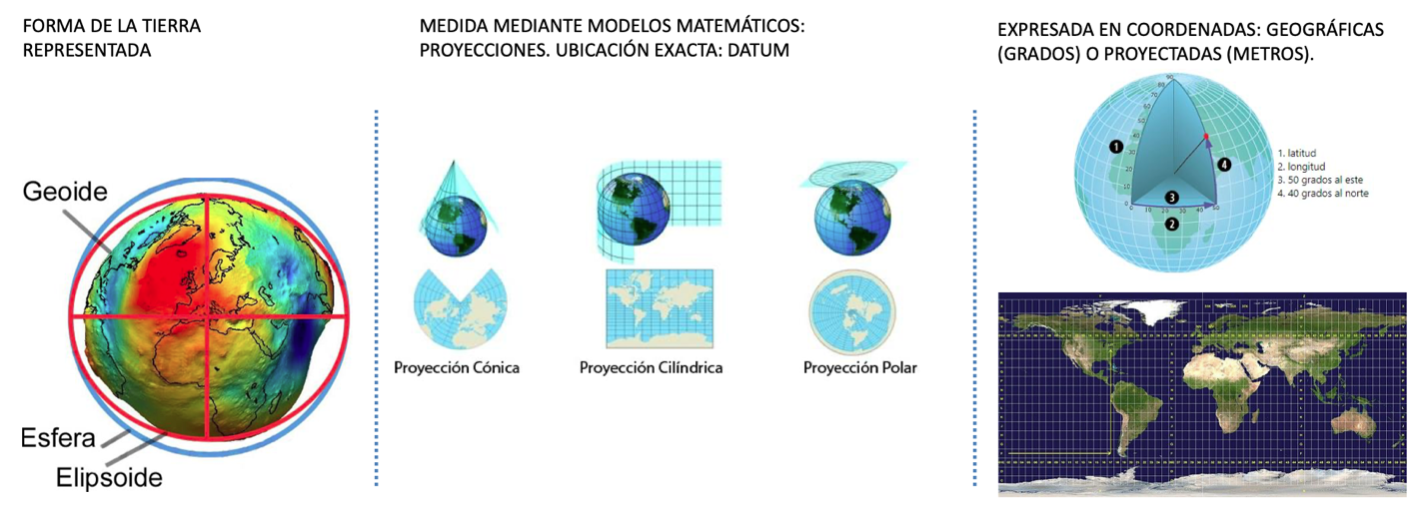
\includegraphics{./images/crs.png}

}

\caption{Sistema de Referencias de Coordenadas}

\end{figure}

Los sistemas de coordenadas forman la base de cálculo para describir la
posición de un punto a partir de mediciones geodésicas: distancias,
proporciones de distancias (sin escala) y ángulos. Las coordenadas nunca
pueden medirse, solamente se calculan con referencia un sistema de
coordenadas bien definido. Los tipos de sistemas de coordenadas
principales que existen son:

\begin{description}
\tightlist
\item[Coordenadas elipsoidales]
son la representación de las coordenadas sobre la superficie de un
elipsoide determinado, se representan por {[}φ, λ, h{]} siendo
respectivamente, la latitud, longitud y altura elipsoidal.
\end{description}

\begin{figure}

{\centering 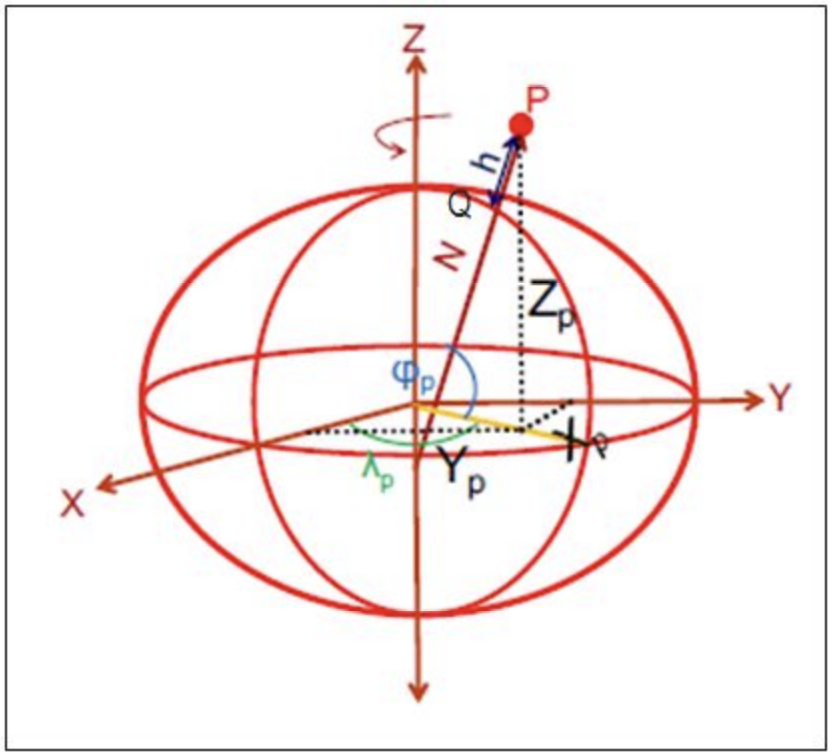
\includegraphics[width=0.6\textwidth,height=\textheight]{./images/geodesicas.png}

}

\caption{Coordenadas Geodésicas. Fuente: (Drewes \& Sánchez, 2011)}

\end{figure}

\begin{description}
\tightlist
\item[Coordenadas proyectadas o cartográficas]
Según la proyección empleada las coordenadas elipsoidales pueden
representarse en un plano, en el caso de Chile continental, se emplea la
proyección Universal Transversal de Mercator (UTM), huso 19 y huso 18.
\end{description}

\begin{figure}

{\centering 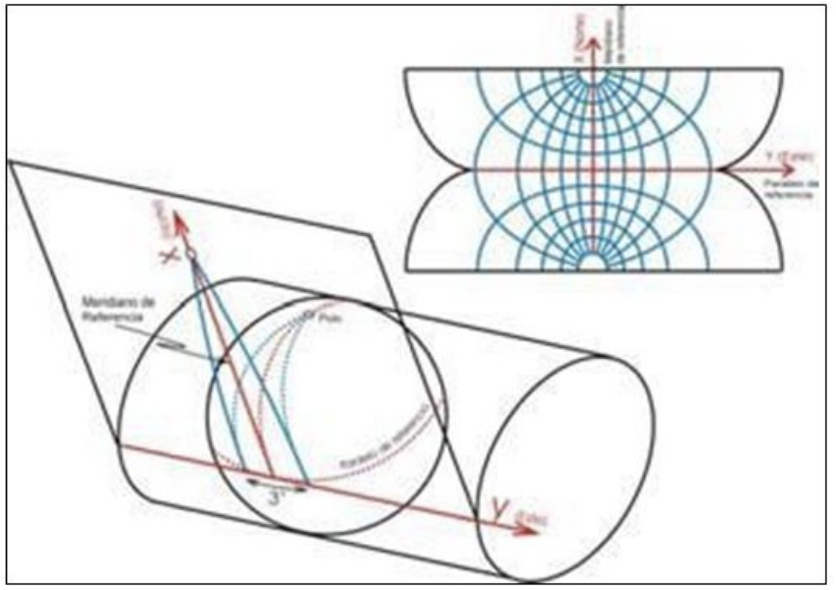
\includegraphics[width=0.6\textwidth,height=\textheight]{./images/utm.png}

}

\caption{proyección Universal Transversal Mercator (UTM) Fuente: (Drewes
\& Sánchez, 2011)}

\end{figure}

Para hacer reproyecciones en R, se le tiene que asignar el Sistema de
Referencia de Coordenadas de dos formas, uno como cadena de texto
(\texttt{"+proj=longlat\ +datum=WGS84\ +no\_defs"}) o como número que
corresponde a EPSG
(\href{https://mappinggis.com/2016/04/los-codigos-epsg-srid-vinculacion-postgis/}{EPSG
es el acrónimo de European Petroleum Survey Group}) que representan
sistema de referencia de coordenadas también.

Para el caso de Chile usamos dos sistemas de referencias de coordenadas:

\begin{description}
\tightlist
\item[Coordenadas elipsoidales (geodésicas):]
4326 o \texttt{"+proj=longlat\ +datum=WGS84\ +no\_defs"}
\item[Coordenadas proyectadas (métricas):]
32719 o
\texttt{"+proj=utm\ +zone=19\ +south\ +datum=WGS84\ +units=m\ +no\_defs"}
\end{description}

\hypertarget{reproyectar-vectores}{%
\subsection{Reproyectar Vectores}\label{reproyectar-vectores}}

\begin{Shaded}
\begin{Highlighting}[]
\NormalTok{LC\_mz\_32719 }\OtherTok{\textless{}{-}}\NormalTok{ las\_condes\_mz }\SpecialCharTok{\%\textgreater{}\%} \FunctionTok{st\_transform}\NormalTok{(}\DecValTok{32719}\NormalTok{)}
\FunctionTok{st\_crs}\NormalTok{(LC\_mz\_32719)}
\end{Highlighting}
\end{Shaded}

\begin{verbatim}
Coordinate Reference System:
  User input: EPSG:32719 
  wkt:
PROJCRS["WGS 84 / UTM zone 19S",
    BASEGEOGCRS["WGS 84",
        ENSEMBLE["World Geodetic System 1984 ensemble",
            MEMBER["World Geodetic System 1984 (Transit)"],
            MEMBER["World Geodetic System 1984 (G730)"],
            MEMBER["World Geodetic System 1984 (G873)"],
            MEMBER["World Geodetic System 1984 (G1150)"],
            MEMBER["World Geodetic System 1984 (G1674)"],
            MEMBER["World Geodetic System 1984 (G1762)"],
            MEMBER["World Geodetic System 1984 (G2139)"],
            ELLIPSOID["WGS 84",6378137,298.257223563,
                LENGTHUNIT["metre",1]],
            ENSEMBLEACCURACY[2.0]],
        PRIMEM["Greenwich",0,
            ANGLEUNIT["degree",0.0174532925199433]],
        ID["EPSG",4326]],
    CONVERSION["UTM zone 19S",
        METHOD["Transverse Mercator",
            ID["EPSG",9807]],
        PARAMETER["Latitude of natural origin",0,
            ANGLEUNIT["degree",0.0174532925199433],
            ID["EPSG",8801]],
        PARAMETER["Longitude of natural origin",-69,
            ANGLEUNIT["degree",0.0174532925199433],
            ID["EPSG",8802]],
        PARAMETER["Scale factor at natural origin",0.9996,
            SCALEUNIT["unity",1],
            ID["EPSG",8805]],
        PARAMETER["False easting",500000,
            LENGTHUNIT["metre",1],
            ID["EPSG",8806]],
        PARAMETER["False northing",10000000,
            LENGTHUNIT["metre",1],
            ID["EPSG",8807]]],
    CS[Cartesian,2],
        AXIS["(E)",east,
            ORDER[1],
            LENGTHUNIT["metre",1]],
        AXIS["(N)",north,
            ORDER[2],
            LENGTHUNIT["metre",1]],
    USAGE[
        SCOPE["Engineering survey, topographic mapping."],
        AREA["Between 72°W and 66°W, southern hemisphere between 80°S and equator, onshore and offshore. Argentina. Bolivia. Brazil. Chile. Colombia. Peru."],
        BBOX[-80,-72,0,-66]],
    ID["EPSG",32719]]
\end{verbatim}

\hypertarget{reproyectar-raster}{%
\subsection{Reproyectar Raster}\label{reproyectar-raster}}

\begin{Shaded}
\begin{Highlighting}[]
\NormalTok{las\_condes\_raster}
\end{Highlighting}
\end{Shaded}

\begin{verbatim}
class      : RasterBrick 
dimensions : 449, 562, 252338, 8  (nrow, ncol, ncell, nlayers)
resolution : 30, 30  (x, y)
extent     : 350505, 367365, 6293905, 6307375  (xmin, xmax, ymin, ymax)
crs        : +proj=utm +zone=19 +south +datum=WGS84 +units=m +no_defs 
source     : OLI_LC.tif 
names      : aerosol,  blue, green,   red,   nir, swir1, swir2, tirs1 
min values :    8465,  7604,  6500,  5924,  5520,  5191,  5197,  5002 
max values :   19119, 20517, 21248, 23237, 29344, 30012, 31166,  5512 
\end{verbatim}

\begin{Shaded}
\begin{Highlighting}[]
\NormalTok{crs\_latlon }\OtherTok{\textless{}{-}} \StringTok{"+proj=longlat +datum=WGS84 +no\_defs"}\CommentTok{\# geográficas o elipsoidales}
\NormalTok{crs\_utm }\OtherTok{\textless{}{-}} \StringTok{"+proj=utm +zone=19 +south +datum=WGS84 +units=m +no\_defs"} \CommentTok{\# UTM o cartográficas}
\NormalTok{las\_condes\_raster2 }\OtherTok{\textless{}{-}} \FunctionTok{projectRaster}\NormalTok{(las\_condes\_raster, }\AttributeTok{crs =}\NormalTok{ crs\_latlon)}
\NormalTok{las\_condes\_raster2}
\end{Highlighting}
\end{Shaded}

\begin{verbatim}
class      : RasterBrick 
dimensions : 470, 578, 271660, 8  (nrow, ncol, ncell, nlayers)
resolution : 0.000323, 0.00027  (x, y)
extent     : -70.61069, -70.424, -33.48775, -33.36085  (xmin, xmax, ymin, ymax)
crs        : +proj=longlat +datum=WGS84 +no_defs 
source     : memory
names      :  aerosol,     blue,    green,      red,      nir,    swir1,    swir2,    tirs1 
min values : 8592.067, 7778.388, 6806.291, 6280.802, 5729.628, 5316.893, 5303.627, 5005.409 
max values : 18590.84, 19485.05, 20596.61, 22406.07, 28732.09, 26707.17, 26787.15,  5495.00 
\end{verbatim}

\hypertarget{actividades-pruxe1cticas}{%
\section{Actividades Prácticas}\label{actividades-pruxe1cticas}}

\begin{enumerate}
\def\labelenumi{\arabic{enumi}.}
\tightlist
\item
  Seleccione una comuna de las manzanas del INE, visualiza con ggplot.
  Además genere una tabla resumen de suma de personas, hombres, mujeres
  viviendas por Zona Censal.
\end{enumerate}

\begin{tcolorbox}[enhanced jigsaw, coltitle=black, colback=white, breakable, toprule=.15mm, left=2mm, opacityback=0, bottomrule=.15mm, colframe=quarto-callout-tip-color-frame, opacitybacktitle=0.6, title=\textcolor{quarto-callout-tip-color}{\faLightbulb}\hspace{0.5em}{Tip}, titlerule=0mm, leftrule=.75mm, bottomtitle=1mm, colbacktitle=quarto-callout-tip-color!10!white, toptitle=1mm, arc=.35mm, rightrule=.15mm]
Leer Archivo:

\begin{Shaded}
\begin{Highlighting}[]
\NormalTok{mz\_ine }\OtherTok{\textless{}{-}} \FunctionTok{readRDS}\NormalTok{(}\StringTok{"../data/censo/manz\_INE\_2017\_sf.rds"}\NormalTok{)}
\end{Highlighting}
\end{Shaded}

Seleccionar Comuna con \texttt{dplyr::filter()}

Eliminar geometrías \texttt{sf::st\_drop\_geometry()} ya que no es
necesaria para realizar tabla resumen.
\end{tcolorbox}

\begin{enumerate}
\def\labelenumi{\arabic{enumi}.}
\setcounter{enumi}{1}
\tightlist
\item
  Visualización de Combinación de Bandas Satelitales
\end{enumerate}

\begin{tcolorbox}[enhanced jigsaw, coltitle=black, colback=white, breakable, toprule=.15mm, left=2mm, opacityback=0, bottomrule=.15mm, colframe=quarto-callout-tip-color-frame, opacitybacktitle=0.6, title=\textcolor{quarto-callout-tip-color}{\faLightbulb}\hspace{0.5em}{Tip}, titlerule=0mm, leftrule=.75mm, bottomtitle=1mm, colbacktitle=quarto-callout-tip-color!10!white, toptitle=1mm, arc=.35mm, rightrule=.15mm]

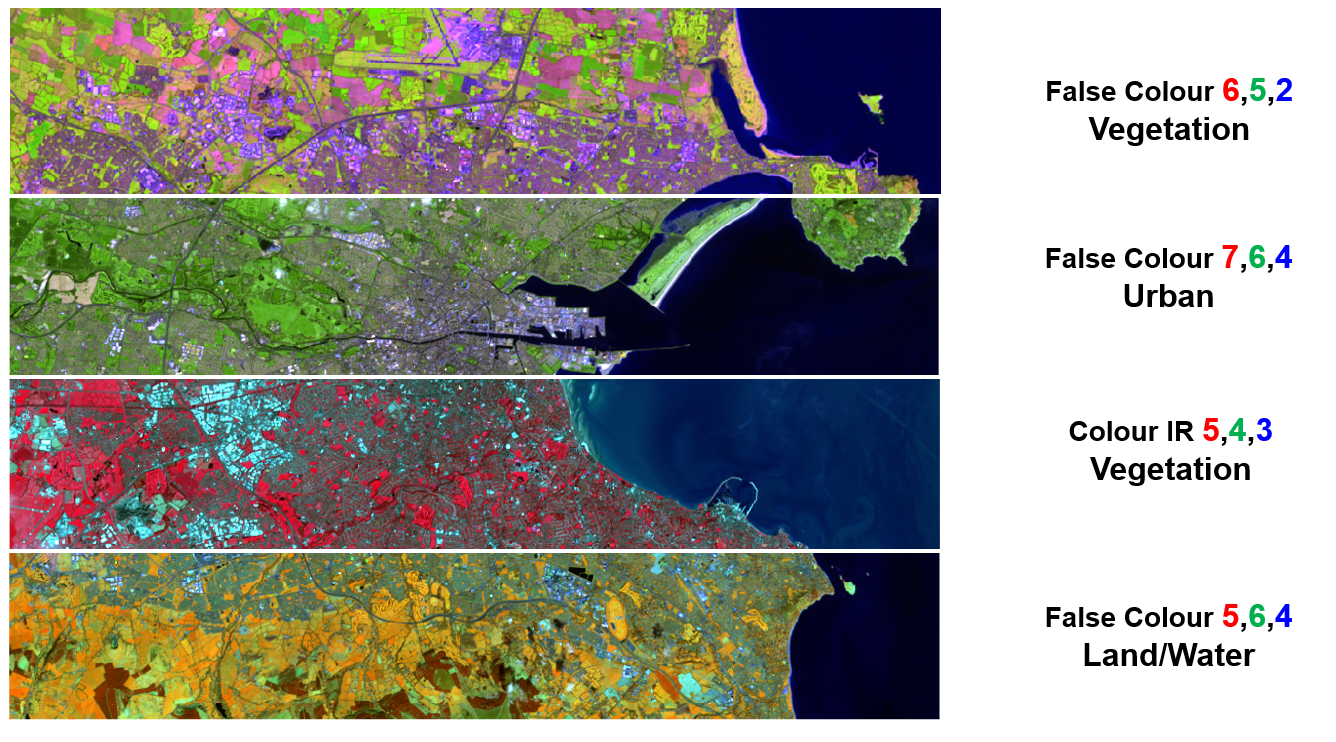
\includegraphics{./images/l8-band-combinations.png} Referencias:
\url{https://mappinggis.com/2019/05/combinaciones-de-bandas-en-imagenes-de-satelite-landsat-y-sentinel/}

\begin{Shaded}
\begin{Highlighting}[]
\FunctionTok{plotRGB}\NormalTok{(las\_condes\_raster, }\AttributeTok{r =} \DecValTok{7}\NormalTok{, }\AttributeTok{g =} \DecValTok{6}\NormalTok{, }\AttributeTok{b =} \DecValTok{4}\NormalTok{, }\AttributeTok{stretch =} \StringTok{"lin"}\NormalTok{)}
\end{Highlighting}
\end{Shaded}

\end{tcolorbox}

\hypertarget{referencias}{%
\section{Referencias}\label{referencias}}

\href{https://www.ide.cl/descargas/Geodesia-en-Chile.pdf}{Geodesia en
Chile, teoría y aplicación del Sistema de Referencia Geocéntrico para
las Américas (SIRGAS) - 2018}

\href{https://r-spatial.github.io/sf/}{Simple Features for R}

\bookmarksetup{startatroot}

\hypertarget{datos-vectoriales-1}{%
\chapter{Datos Vectoriales}\label{datos-vectoriales-1}}

Módulo 2: Práctico

\hfill\break

\begin{itemize}
\tightlist
\item
  Manipulación de Datos Vectoriales
\item
  Definición de Indicadores Territoriales
\item
  Construcción de Indicadores Socioeconómicos
\end{itemize}

\hypertarget{manipulaciuxf3n-de-datos-vectoriales}{%
\section{Manipulación de Datos
Vectoriales}\label{manipulaciuxf3n-de-datos-vectoriales}}

\begin{itemize}
\tightlist
\item
  Lectura
\item
  Reproyectar CRS
\item
  Filtros
\item
  Buffer Espacial
\item
  Resumen Estadísticos
\item
  Joining
\end{itemize}

\hypertarget{lectura-de-insumos}{%
\subsection{Lectura de Insumos}\label{lectura-de-insumos}}

Para los efectos prácticos de esta etapa se utilizarà la base de datos
del censo a nivel zonal a nivel nacional.

\begin{Shaded}
\begin{Highlighting}[]
\NormalTok{zonas\_censales }\OtherTok{\textless{}{-}}  \FunctionTok{readRDS}\NormalTok{(}\StringTok{"data/censo/zonas\_urb\_consolidadas.rds"}\NormalTok{)}
\NormalTok{zonas\_censales}
\end{Highlighting}
\end{Shaded}

\begin{verbatim}
Simple feature collection with 4865 features and 22 fields
Geometry type: MULTIPOLYGON
Dimension:     XY
Bounding box:  xmin: -109.4441 ymin: -54.93931 xmax: -67.58767 ymax: -18.19346
CRS:           +proj=longlat +datum=WGS84 +ellps=WGS84 +towgs84=0,0,0
First 10 features:
   REGION         NOM_REGION PROVINCIA NOM_PROVIN COMUNA    NOM_COMUNA
1       1 REGIÓN DE TARAPACÁ        14  TAMARUGAL   1405          PICA
2       1 REGIÓN DE TARAPACÁ        14  TAMARUGAL   1401  POZO ALMONTE
3       1 REGIÓN DE TARAPACÁ        14  TAMARUGAL   1401  POZO ALMONTE
4       1 REGIÓN DE TARAPACÁ        14  TAMARUGAL   1404         HUARA
5       1 REGIÓN DE TARAPACÁ        11    IQUIQUE   1107 ALTO HOSPICIO
6       1 REGIÓN DE TARAPACÁ        11    IQUIQUE   1107 ALTO HOSPICIO
7       1 REGIÓN DE TARAPACÁ        11    IQUIQUE   1107 ALTO HOSPICIO
8       1 REGIÓN DE TARAPACÁ        11    IQUIQUE   1107 ALTO HOSPICIO
9       1 REGIÓN DE TARAPACÁ        11    IQUIQUE   1107 ALTO HOSPICIO
10      1 REGIÓN DE TARAPACÁ        11    IQUIQUE   1107 ALTO HOSPICIO
          URBANO DISTRITO LOC_ZON  GEOCODIGO      AREA COD_INE_15 COD_INE_16
1           PICA        1       1 1405011001 9336400.3 1405011001 1405011001
2   POZO ALMONTE        1       1 1401011001 1941994.2 1401011001 1401011001
3   POZO ALMONTE        1       2 1401011002 3572254.9 1401011002 1401011002
4          HUARA        1       1 1404011001  603314.2 1404011001 1404011001
5  ALTO HOSPICIO        1       2 1107011002 2272129.2 1107011002 1107011002
6  ALTO HOSPICIO        3       2 1107031002 5820325.8 1107031002 1107031002
7  ALTO HOSPICIO        1       3 1107011003 5390203.8 1107011003 1107011003
8  ALTO HOSPICIO        2       4 1107021004  461102.3 1107021004 1107021004
9  ALTO HOSPICIO        2       1 1107021001 1018532.8 1107021001 1107021001
10 ALTO HOSPICIO        2       2 1107021002  533877.5 1107021002 1107021002
   VALIDO       KM2    ESC_JH PERS      M2_O      M2_C   DENS_HAB   DENS_OF
1    TRUE 9.3364003 10.817377 3876    0.0000    0.0000   415.1493    0.0000
2    TRUE 1.9419942 10.224880 2771 1476.0000 4093.0000  1426.8838  760.0435
3    TRUE 3.5722549 10.253158 6506 1905.0000 9696.0000  1821.2586  533.2766
4    TRUE 0.6033142  9.523220 1082    0.0000    0.0000  1793.4270    0.0000
5    TRUE 2.2721292  9.747321 4360  475.0686  180.6789  1918.9050  209.0852
6    TRUE 5.8203258  9.397516 7099 4003.6214 1008.7833  1219.6912  687.8690
7    TRUE 5.3902038 10.191809 8549 2024.1914 1619.3701  1586.0254  375.5315
8    TRUE 0.4611023 10.734940 5125  875.3943 5843.4606 11114.6691 1898.4815
9    TRUE 1.0185328  9.277910 6701  156.0181 1792.1965  6579.0714  153.1793
10   TRUE 0.5338775  9.723104 3971 1020.3947 9931.7124  7438.0352 1911.2897
      DENS_COM                       geometry
1      0.00000 MULTIPOLYGON (((-69.31192 -...
2   2107.62731 MULTIPOLYGON (((-69.78591 -...
3   2714.25201 MULTIPOLYGON (((-69.76215 -...
4      0.00000 MULTIPOLYGON (((-69.7696 -1...
5     79.51965 MULTIPOLYGON (((-70.09246 -...
6    173.32076 MULTIPOLYGON (((-70.05305 -...
7    300.42836 MULTIPOLYGON (((-70.06791 -...
8  12672.80609 MULTIPOLYGON (((-70.10537 -...
9   1759.58643 MULTIPOLYGON (((-70.10938 -...
10 18602.97808 MULTIPOLYGON (((-70.09582 -...
\end{verbatim}

\hypertarget{tbl-censo-zonas}{}
\begin{table}
\caption{\label{tbl-censo-zonas}Registros de Zonas Censales del Censo 2017 }\tabularnewline

\centering\begingroup\fontsize{8}{10}\selectfont

\begin{tabular}[t]{l|l|l|l|l|l|l|r|r|l|r|r|r|l|r|r|r|r|r|r|r|r|l}
\hline
REGION & NOM\_REGION & PROVINCIA & NOM\_PROVIN & COMUNA & NOM\_COMUNA & URBANO & DISTRITO & LOC\_ZON & GEOCODIGO & AREA & COD\_INE\_15 & COD\_INE\_16 & VALIDO & KM2 & ESC\_JH & PERS & M2\_O & M2\_C & DENS\_HAB & DENS\_OF & DENS\_COM & geometry\\
\hline
1 & REGIÓN DE TARAPACÁ & 14 & TAMARUGAL & 1405 & PICA & PICA & 1 & 1 & 1405011001 & 9336400.3 & 1405011001 & 1405011001 & TRUE & 9.3364003 & 10.817377 & 3876 & 0.0000 & 0.0000 & 415.1493 & 0.0000 & 0.00000 & MULTIPOLYGON (((-69.31192 -...\\
\hline
1 & REGIÓN DE TARAPACÁ & 14 & TAMARUGAL & 1401 & POZO ALMONTE & POZO ALMONTE & 1 & 1 & 1401011001 & 1941994.2 & 1401011001 & 1401011001 & TRUE & 1.9419942 & 10.224880 & 2771 & 1476.0000 & 4093.0000 & 1426.8838 & 760.0435 & 2107.62731 & MULTIPOLYGON (((-69.78591 -...\\
\hline
1 & REGIÓN DE TARAPACÁ & 14 & TAMARUGAL & 1401 & POZO ALMONTE & POZO ALMONTE & 1 & 2 & 1401011002 & 3572254.9 & 1401011002 & 1401011002 & TRUE & 3.5722549 & 10.253158 & 6506 & 1905.0000 & 9696.0000 & 1821.2586 & 533.2766 & 2714.25201 & MULTIPOLYGON (((-69.76215 -...\\
\hline
1 & REGIÓN DE TARAPACÁ & 14 & TAMARUGAL & 1404 & HUARA & HUARA & 1 & 1 & 1404011001 & 603314.2 & 1404011001 & 1404011001 & TRUE & 0.6033142 & 9.523220 & 1082 & 0.0000 & 0.0000 & 1793.4270 & 0.0000 & 0.00000 & MULTIPOLYGON (((-69.7696 -1...\\
\hline
1 & REGIÓN DE TARAPACÁ & 11 & IQUIQUE & 1107 & ALTO HOSPICIO & ALTO HOSPICIO & 1 & 2 & 1107011002 & 2272129.2 & 1107011002 & 1107011002 & TRUE & 2.2721292 & 9.747321 & 4360 & 475.0686 & 180.6789 & 1918.9050 & 209.0852 & 79.51965 & MULTIPOLYGON (((-70.09246 -...\\
\hline
1 & REGIÓN DE TARAPACÁ & 11 & IQUIQUE & 1107 & ALTO HOSPICIO & ALTO HOSPICIO & 3 & 2 & 1107031002 & 5820325.8 & 1107031002 & 1107031002 & TRUE & 5.8203258 & 9.397516 & 7099 & 4003.6214 & 1008.7833 & 1219.6912 & 687.8690 & 173.32076 & MULTIPOLYGON (((-70.05305 -...\\
\hline
\end{tabular}
\endgroup{}
\end{table}

\hypertarget{reproyectar-crs}{%
\subsection{Reproyectar CRS}\label{reproyectar-crs}}

\hypertarget{filtros}{%
\subsection{Filtros}\label{filtros}}

\hypertarget{buffer-espacial}{%
\subsection{Buffer Espacial}\label{buffer-espacial}}

\hypertarget{resumen-estaduxedsticos}{%
\subsection{Resumen Estadísticos}\label{resumen-estaduxedsticos}}

\hypertarget{joining}{%
\subsection{Joining}\label{joining}}

\hypertarget{indicadores-territoriales}{%
\section{Indicadores Territoriales}\label{indicadores-territoriales}}

\hypertarget{definiciuxf3n-de-indicadores}{%
\subsection{Definición de
Indicadores}\label{definiciuxf3n-de-indicadores}}

\begin{description}
\item[¿Qué es un Indicador?:]
Un indicador es un instrumento que provee información de una determinada
condición, situación, actividad o resultado. Este instrumento nos
permite definir un punto de comparación para establecer diferencias
entre individuos o respecto a sí mismo en diferentes tiempos. Son
construidos a través de análisis y operaciones técnicas y nos entregan
una medida cuantitativa (valor) o una descripción cualitativa
(caracterización) de la magnitud o criterio que se pretende medir u
observar.
\end{description}

\hypertarget{indicadores-territoriales-1}{%
\subsection{Indicadores
Territoriales}\label{indicadores-territoriales-1}}

El Centro de Inteligencia Territorial de la Universidad Adolfo Ibañez,
bajo proyecto denominado \textbf{Matriz de Bienestar Humano Territorial
(MBHT)} construyó una serie indicadores territoriales, que buscan
comprender las condiciones de los entornos urbanos y rurales, para
construir soluciones que impacten positivamente en el bienestar de las
personas y su hábitat.

\begin{figure}

{\centering 


\includegraphics[width=0.3\textwidth,height=\textheight]{./images/Logo_CIT_UAI_Negro.png}
\includegraphics[width=0.18\textwidth,height=\textheight]{./images/logo-mbht.png}

}

\caption{\label{fig-cit}Centro de Inteligencia Territorial - UAI}

\end{figure}

El sistema MBHT consiste en 18 indicadores territoriales agrupados en 4
dimensiones, que corresponde a las dimensiones de Accesibilidad,
Ambiental, Seguridad y Socoeconómicas, siendo esta última a la se
replicará.

\begin{figure}

{\centering 

\begin{figure}

{\centering 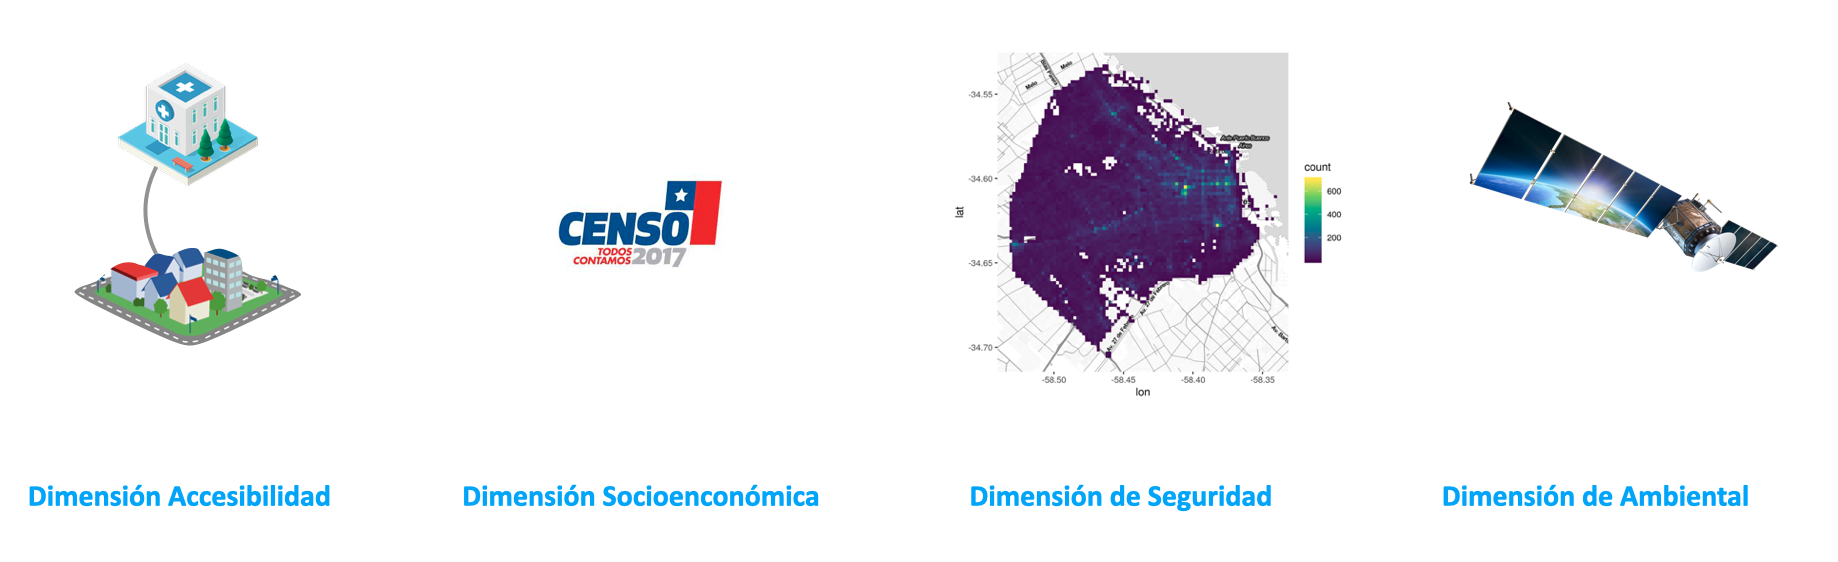
\includegraphics{./images/dimensiones_bht.png}

}

\end{figure}

}

\caption{\label{fig-mbht}Dimensiones de la Matriz de Bienestar Humano
Territorial}

\end{figure}

\hypertarget{construcciuxf3n-de-indicadores-socioconuxf3micos}{%
\section{Construcción de Indicadores
Socioconómicos}\label{construcciuxf3n-de-indicadores-socioconuxf3micos}}

Las ciudades de Chile presentan altos índices de segregación (Sabatini,
2002), que reflejan la separación espacial de distintos grupos sociales
(Ruiz-Tagle, 2014). La intensidad de este fenómeno hace imperativo el
considerar la condición social como una dimensión estructurante en la
evaluación de Políticas Públicas.

\begin{figure}

{\centering 

\begin{figure}

{\centering 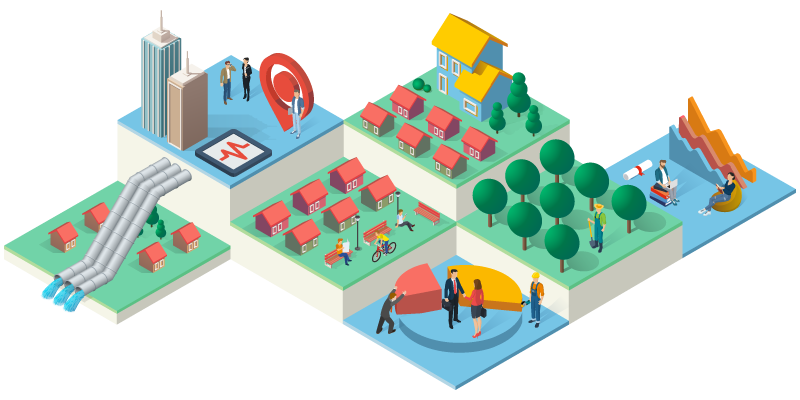
\includegraphics[width=0.4\textwidth,height=\textheight]{./images/socioeconomico.png}

}

\end{figure}

}

\caption{\label{fig-soc-mbht}Indicadores Socioconómicos}

\end{figure}

\hypertarget{insumos-censo-2017}{%
\subsection{Insumos Censo 2017}\label{insumos-censo-2017}}

Para la construcción de los indicadores territoriales que componen la
dimensión seocioeconómica, se utiliza integramente información del Censo
2017.

\textbf{¿Que es Censo 2017?:}

El censo de población y vivienda es la operación estadística más
importante que realiza el INE y en la cual participan todos los
habitantes del país, ya que este es un insumo esencial para elaborar
estimaciones y proyecciones de población tanto para el país, las
regiones y las comunas.

El censo permite contar con información esencial para el adecuado diseño
de políticas públicas y toma de decisiones privadas y públicas. El
último censo de población y vivienda realizado fue en 2017. Sus
resultados indican que la población efectivamente censada llegó a un
total de 17.574.003 personas.

De ellas, 8.601.989 (48,9\%) son hombres y 8.972.014 (51,1\%), mujeres.
El número de viviendas, en tanto, fue 6.499.355, de las cuales 6.486.533
(99,8\%) corresponden a viviendas particulares y 12.822 (0,2\%) a
colectivas.

Para estos fines, se utilizaremos información censal agregada a nivel de
\textbf{manzanas} obtenidos del Censo 2017, a continuación se explorará
los insumos utilizados.

\begin{figure}

{\centering 

\begin{figure}

{\centering 
\includegraphics[width=0.2\textwidth,height=\textheight]{./images/censo_2017.png}

}

\end{figure}

}

\caption{\label{fig-logo-censo}Censo 2017 - Instituto Nacional de
Estadísticas de Chile}

\end{figure}

\hypertarget{insumos-del-censo}{%
\subsection{Insumos del Censo}\label{insumos-del-censo}}

Pa los indicadores que se crearàn a continuación se tilizará una base
proveniente de la consolidación de las bases del censo, demoninadas
microdatos de Personas, Viviendas y Hogares provenientes de los
resultados de la Encuensta del Censo 2017 del Instituto Nacional de
Estadísticas, Chile.

\begin{Shaded}
\begin{Highlighting}[]
\FunctionTok{library}\NormalTok{(sf)}
\FunctionTok{library}\NormalTok{(dplyr)}

\CommentTok{\# ruta de insumos}
\NormalTok{path\_insumos }\OtherTok{\textless{}{-}} \StringTok{"data/socioeconomicos/insumos/"}
\end{Highlighting}
\end{Shaded}

Lectura de Insumos y selección de región de estudio, en este caso
seleccionará la
\href{https://es.wikipedia.org/wiki/Región_de_Coquimbo}{Región de
Coquimbo} compuesta por las provincias de Elqui, Limarí y Choapa. Sus
principales centros urbanos son la Conurbación La Serena-Coquimbo con
506 391 habitantes, seguida de Ovalle con 121.269 habitantes según el
Censo chileno de 2017.

\begin{Shaded}
\begin{Highlighting}[]
\CommentTok{\# selección de región}
\NormalTok{reg }\OtherTok{\textless{}{-}}  \StringTok{"R04"}

\CommentTok{\# Lectura de insumo espacial}
\NormalTok{path\_file }\OtherTok{\textless{}{-}} \FunctionTok{paste0}\NormalTok{(path\_insumos, reg, }\StringTok{"\_INSUMO\_SOCIOECONOMICO.shp"}\NormalTok{)}
\NormalTok{censo }\OtherTok{\textless{}{-}} \FunctionTok{st\_read}\NormalTok{(path\_file, }\AttributeTok{quiet =}\NormalTok{ T)}
\end{Highlighting}
\end{Shaded}

\textbf{Visualización de Tabla de Información \texttt{head()}}

\hypertarget{tbl-censo}{}
\begin{table}
\caption{\label{tbl-censo}Visualización de registros de insumos del Censo 2017 para indicadores
socioeconómicos }\tabularnewline

\centering\begingroup\fontsize{8}{10}\selectfont

\begin{tabular}[t]{l|l|l|r|l|r|l|r|l|l|r|r|r|r|r|r|r|r|r|r|r|r|r|r|r|r|r|r|r|r|r|r|r|r|r|l}
\hline
ID\_MANZ & MANZ\_EN & NOM\_COM & COD\_COM & NOM\_REG & COD\_REG & NOM\_PROV & COD\_PROV & ZONA & ID\_MANZCIT & AREA & TOTAL\_V & HOG\_N & PERSONAS & E4A18 & E15A24 & ESCOLAR & P03A\_4 & P03A\_5 & P03A\_6 & P03B\_4 & P03B\_6 & P03B\_7 & P03C\_4 & P03C\_5 & NIV\_HAC2 & NIV\_HAC3 & HOMBRES & MUJERES & MONOPAR & P17\_ACT & P17\_4 & J\_NINI & JH\_HASTA\_P & JH\_HASTA\_S & geometry\\
\hline
4101071001900 & URBANO & LA SERENA & 4101 & REGIÓN DE COQUIMBO & 4 & ELQUI & 41 & 4101071001 & 4101071001900001 & 2873.376 & 0 & 0 & 0 & 0 & 0 & 0 & 0 & 0 & 0 & 0 & 0 & 0 & 0 & 0 & 0 & 0 & 0 & 0 & 0 & 0 & 0 & 0 & 0 & 0 & POLYGON ((292811 6685815, 2...\\
\hline
4101071001900 & URBANO & LA SERENA & 4101 & REGIÓN DE COQUIMBO & 4 & ELQUI & 41 & 4101071001 & 4101071001900002 & 1256.480 & 0 & 0 & 0 & 0 & 0 & 0 & 0 & 0 & 0 & 0 & 0 & 0 & 0 & 0 & 0 & 0 & 0 & 0 & 0 & 0 & 0 & 0 & 0 & 0 & POLYGON ((293056 6685511, 2...\\
\hline
4102101001900 & URBANO & COQUIMBO & 4102 & REGIÓN DE COQUIMBO & 4 & ELQUI & 41 & 4102101001 & 4102101001900001 & 1230.344 & 0 & 0 & 0 & 0 & 0 & 0 & 0 & 0 & 0 & 0 & 0 & 0 & 0 & 0 & 0 & 0 & 0 & 0 & 0 & 0 & 0 & 0 & 0 & 0 & POLYGON ((285917.8 6664517,...\\
\hline
4102101001900 & URBANO & COQUIMBO & 4102 & REGIÓN DE COQUIMBO & 4 & ELQUI & 41 & 4102101001 & 4102101001900002 & 3877.142 & 0 & 0 & 0 & 0 & 0 & 0 & 0 & 0 & 0 & 0 & 0 & 0 & 0 & 0 & 0 & 0 & 0 & 0 & 0 & 0 & 0 & 0 & 0 & 0 & POLYGON ((286085 6664254, 2...\\
\hline
4102101001900 & URBANO & COQUIMBO & 4102 & REGIÓN DE COQUIMBO & 4 & ELQUI & 41 & 4102101001 & 4102101001900003 & 34392.873 & 0 & 0 & 0 & 0 & 0 & 0 & 0 & 0 & 0 & 0 & 0 & 0 & 0 & 0 & 0 & 0 & 0 & 0 & 0 & 0 & 0 & 0 & 0 & 0 & POLYGON ((286082.4 6663489,...\\
\hline
4106101001900 & URBANO & VICUÑA & 4106 & REGIÓN DE COQUIMBO & 4 & ELQUI & 41 & 4106101001 & 4106101001900001 & 4033.107 & 0 & 0 & 0 & 0 & 0 & 0 & 0 & 0 & 0 & 0 & 0 & 0 & 0 & 0 & 0 & 0 & 0 & 0 & 0 & 0 & 0 & 0 & 0 & 0 & POLYGON ((310231.6 6684580,...\\
\hline
\end{tabular}
\endgroup{}
\end{table}

\hypertarget{indicador-de-escolaridad-del-jefe-de-hogar-iej}{%
\section{Indicador de Escolaridad del jefe de hogar
(IEJ)}\label{indicador-de-escolaridad-del-jefe-de-hogar-iej}}

Para la construcción de este indicador se utilizó el promedio de años de
estudio de jefes de hogar (EJH), que es una variable censal numérica
(``ESCOLARIDAD'', en tabla de personas del censo 2017) que registra el
nivel del curso más alto aprobado, medida en años sucesivos desde la
enseñanza básica hasta estudios de postgrado.

Se calcula el promedio de esta variable para todos los jefes de hogar en
cada manzana. Esta variable es representativa del capital cultural de
cada hogar y está altamente correlacionada con el nivel de ingresos en
Chile (Agostini et al, 2016).

** Cálculo Indicador de Escolaridad del jefe de hogar (IEJ)**

\begin{Shaded}
\begin{Highlighting}[]
\NormalTok{censo }\OtherTok{\textless{}{-}}\NormalTok{ censo }\SpecialCharTok{\%\textgreater{}\%} \FunctionTok{mutate}\NormalTok{( }\AttributeTok{IEJ =}\NormalTok{ ESCOLAR)}
\end{Highlighting}
\end{Shaded}

Para efectos de visualización se enfocará los resultados en las zonas
urbanas de la comuna de La Serena en todos los indicadores que se
presentarán.

\begin{Shaded}
\begin{Highlighting}[]
\NormalTok{la\_serena\_urb }\OtherTok{\textless{}{-}}\NormalTok{ censo }\SpecialCharTok{\%\textgreater{}\%} \FunctionTok{filter}\NormalTok{(COD\_COM }\SpecialCharTok{==} \DecValTok{4101} \SpecialCharTok{\&}\NormalTok{ MANZ\_EN }\SpecialCharTok{==} \StringTok{"URBANO"}\NormalTok{)}
\end{Highlighting}
\end{Shaded}

\textbf{Visualizar la Variable de \texttt{IEJ} comuna de La Serena
\texttt{URBANO}}:

\begin{Shaded}
\begin{Highlighting}[]
\FunctionTok{ggplot}\NormalTok{() }\SpecialCharTok{+}
  \FunctionTok{geom\_sf}\NormalTok{(}\AttributeTok{data =}\NormalTok{ la\_serena\_urb, }\FunctionTok{aes}\NormalTok{(}\AttributeTok{fill =}\NormalTok{ IEJ), }\AttributeTok{color =}\ConstantTok{NA}\NormalTok{, }
          \AttributeTok{alpha=}\FloatTok{0.8}\NormalTok{,  }\AttributeTok{size=} \FloatTok{0.1}\NormalTok{)}\SpecialCharTok{+}
  \FunctionTok{scale\_fill\_distiller}\NormalTok{(}\AttributeTok{palette=} \StringTok{"YlGnBu"}\NormalTok{, }\AttributeTok{direction =} \DecValTok{1}\NormalTok{)}\SpecialCharTok{+}
  \FunctionTok{ggtitle}\NormalTok{(}\StringTok{"Indicador de Escolaridad del jefe de hogar (IEJ) {-} Urbano"}\NormalTok{ ) }\SpecialCharTok{+}
  \FunctionTok{theme\_bw}\NormalTok{() }\SpecialCharTok{+}
  \FunctionTok{theme}\NormalTok{(}\AttributeTok{panel.grid.major =} \FunctionTok{element\_line}\NormalTok{(}\AttributeTok{colour =} \StringTok{"gray80"}\NormalTok{), }
        \AttributeTok{panel.grid.minor =} \FunctionTok{element\_line}\NormalTok{(}\AttributeTok{colour =} \StringTok{"gray80"}\NormalTok{))}
\end{Highlighting}
\end{Shaded}

\begin{figure}[H]

{\centering 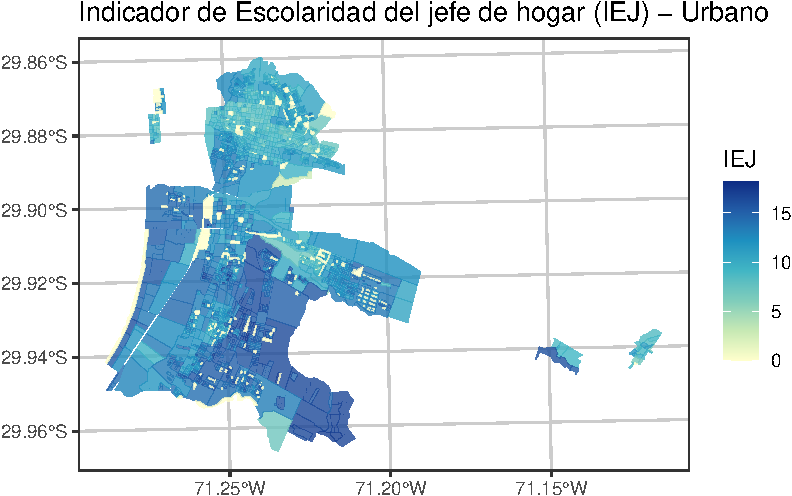
\includegraphics{./datos_vectoriales_files/figure-pdf/fig-iej-urbano-1.pdf}

}

\caption{\label{fig-iej-urbano}Indicador de Escolaridad del jefe de
hogar (IEJ) - Urbano}

\end{figure}

\begin{Shaded}
\begin{Highlighting}[]
\CommentTok{\# mapview::mapview(censo \%\textgreater{}\% filter(COD\_COM == 4101 \& MANZ\_EN == "URBANO"),}
                 \CommentTok{\# zcol = "IEJ", layer.name = "IEJ")}
\end{Highlighting}
\end{Shaded}

\textbf{Visualizar la Variable de \texttt{IEJ} comuna de La Serena
\texttt{RURAL}}:

\begin{Shaded}
\begin{Highlighting}[]
\NormalTok{la\_serena\_rural }\OtherTok{\textless{}{-}}\NormalTok{ censo }\SpecialCharTok{\%\textgreater{}\%} \FunctionTok{filter}\NormalTok{(COD\_COM }\SpecialCharTok{==} \DecValTok{4101} \SpecialCharTok{\&}\NormalTok{ MANZ\_EN }\SpecialCharTok{==} \StringTok{"RURAL"}\NormalTok{)}

\FunctionTok{ggplot}\NormalTok{() }\SpecialCharTok{+}
  \FunctionTok{geom\_sf}\NormalTok{(}\AttributeTok{data =}\NormalTok{ la\_serena\_rural, }\FunctionTok{aes}\NormalTok{(}\AttributeTok{fill =}\NormalTok{ IEJ), }\AttributeTok{color =}\ConstantTok{NA}\NormalTok{, }
          \AttributeTok{alpha=}\FloatTok{0.8}\NormalTok{,  }\AttributeTok{size=} \FloatTok{0.1}\NormalTok{)}\SpecialCharTok{+}
  \FunctionTok{scale\_fill\_distiller}\NormalTok{(}\AttributeTok{palette=} \StringTok{"YlGnBu"}\NormalTok{, }\AttributeTok{direction =} \DecValTok{1}\NormalTok{)}\SpecialCharTok{+}
  \FunctionTok{ggtitle}\NormalTok{(}\StringTok{"Indicador de Escolaridad del jefe de hogar (IEJ) {-} Rural"}\NormalTok{ ) }\SpecialCharTok{+}
  \FunctionTok{theme\_bw}\NormalTok{() }\SpecialCharTok{+}
  \FunctionTok{theme}\NormalTok{(}\AttributeTok{panel.grid.major =} \FunctionTok{element\_line}\NormalTok{(}\AttributeTok{colour =} \StringTok{"gray80"}\NormalTok{), }
        \AttributeTok{panel.grid.minor =} \FunctionTok{element\_line}\NormalTok{(}\AttributeTok{colour =} \StringTok{"gray80"}\NormalTok{))}
\CommentTok{\# mapview::mapview(censo \%\textgreater{}\% filter(COD\_COM == 4101 \& MANZ\_EN == "RURAL"),}
                 \CommentTok{\# zcol = "IEJ", layer.name = "IEJ")}
\end{Highlighting}
\end{Shaded}

\begin{figure}[H]

{\centering 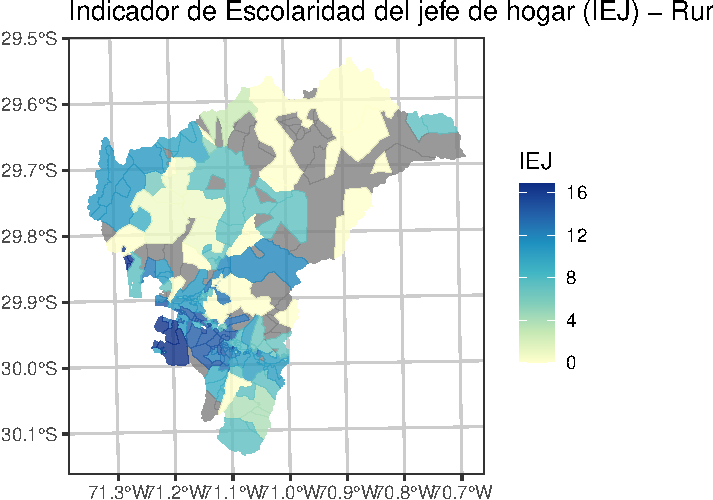
\includegraphics{./datos_vectoriales_files/figure-pdf/fig-iej-rural-1.pdf}

}

\caption{\label{fig-iej-rural}Indicador de Escolaridad del jefe de hogar
(IEJ) - Rural}

\end{figure}

\hypertarget{indicador-de-empleo-iem}{%
\section{Indicador de Empleo (IEM)}\label{indicador-de-empleo-iem}}

Para este indicador se usó la proporción de población activa sin empleo
que es la fracción de las personas que no tienen empleo y están buscando
uno, respecto al total de personas en condiciones y con deseo de
trabajar en cada manzana.

Esta variable es similar al cálculo de desempleo, pero calculada a
escala de manzanas y en un tiempo específico, por lo que representa las
brechas potenciales que existen para acceder al empleo en barrios
específicos (MDS, 2019).

** Cálculo Indicador de Empleo (IEM) **

\textbf{P17\_4}: Trabajo la semana pasada, \emph{opción 4}: ``Se
encontraba buscando empleo''\\
\textbf{P17\_ACT}: Total de Actividades Remuneradas (no es pregunta del
Censo)

\begin{Shaded}
\begin{Highlighting}[]
\CommentTok{\# P17: Trabajo la semana pasada}
\CommentTok{\# opción \textasciigrave{}4\textasciigrave{}: "Se encontraba buscando empleo"}
\CommentTok{\# P17\_ACT: Total de Actividades Remuneradas}

\NormalTok{censo }\OtherTok{\textless{}{-}}\NormalTok{ censo }\SpecialCharTok{\%\textgreater{}\%} \FunctionTok{mutate}\NormalTok{( }\AttributeTok{CESA\_DENS =}\NormalTok{ P17\_4 }\SpecialCharTok{/}\NormalTok{ P17\_ACT)}

\CommentTok{\# Invetir el valor de indicador 1}
\NormalTok{censo }\OtherTok{\textless{}{-}}\NormalTok{ censo }\SpecialCharTok{\%\textgreater{}\%} \FunctionTok{mutate}\NormalTok{( }\AttributeTok{IEM =} \DecValTok{1} \SpecialCharTok{{-}}\NormalTok{ CESA\_DENS )}
\end{Highlighting}
\end{Shaded}

De aquí continiuación se realizaràn cartografías solo a zonas urbanas a
efecto de limitar la extensión del presente documento, pero el cáculo
urbano se puede efectuar perfectamente aplicando un filtro como se
ejemplifico en el indicador anterior. Ahora, se procede a filtrar por
zonas urbanas

\begin{Shaded}
\begin{Highlighting}[]
\NormalTok{la\_serena\_urb }\OtherTok{\textless{}{-}}\NormalTok{ censo }\SpecialCharTok{\%\textgreater{}\%} \FunctionTok{filter}\NormalTok{(COD\_COM }\SpecialCharTok{==} \DecValTok{4101} \SpecialCharTok{\&}\NormalTok{ MANZ\_EN }\SpecialCharTok{==} \StringTok{"URBANO"}\NormalTok{)}
\end{Highlighting}
\end{Shaded}

\textbf{Visualizar la Variable de \texttt{IEM} comuna de La Serena
\texttt{URBANO}}:

\begin{Shaded}
\begin{Highlighting}[]
\FunctionTok{ggplot}\NormalTok{() }\SpecialCharTok{+}
  \FunctionTok{geom\_sf}\NormalTok{(}\AttributeTok{data =}\NormalTok{ la\_serena\_urb, }\FunctionTok{aes}\NormalTok{(}\AttributeTok{fill =}\NormalTok{ IEM), }\AttributeTok{color =}\ConstantTok{NA}\NormalTok{, }
          \AttributeTok{alpha=}\FloatTok{0.8}\NormalTok{,  }\AttributeTok{size=} \FloatTok{0.1}\NormalTok{)}\SpecialCharTok{+}
  \FunctionTok{scale\_fill\_distiller}\NormalTok{(}\AttributeTok{palette=} \StringTok{"PuBu"}\NormalTok{, }\AttributeTok{direction =} \DecValTok{1}\NormalTok{)}\SpecialCharTok{+}
  \FunctionTok{ggtitle}\NormalTok{(}\StringTok{"Indicador de Empleo (IEM) {-} Urbano"}\NormalTok{ ) }\SpecialCharTok{+}
  \FunctionTok{theme\_bw}\NormalTok{() }\SpecialCharTok{+}
  \FunctionTok{theme}\NormalTok{(}\AttributeTok{panel.grid.major =} \FunctionTok{element\_line}\NormalTok{(}\AttributeTok{colour =} \StringTok{"gray80"}\NormalTok{), }
        \AttributeTok{panel.grid.minor =} \FunctionTok{element\_line}\NormalTok{(}\AttributeTok{colour =} \StringTok{"gray80"}\NormalTok{))}
\end{Highlighting}
\end{Shaded}

\begin{figure}[H]

{\centering 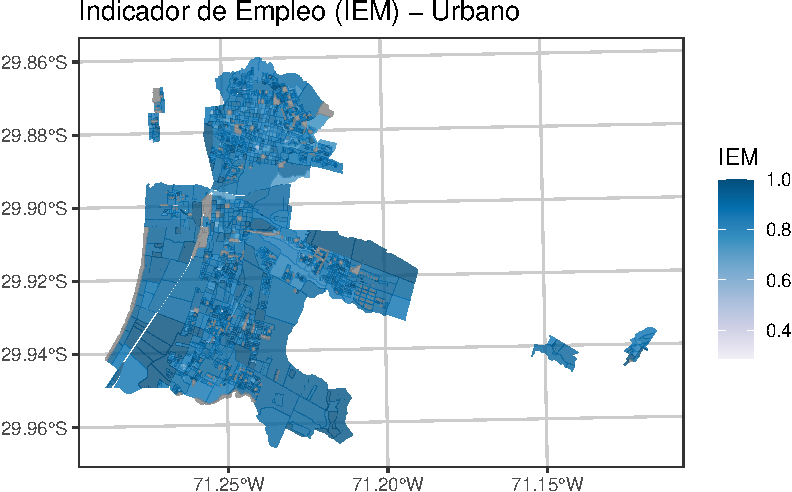
\includegraphics{./datos_vectoriales_files/figure-pdf/fig-iem-urbano-1.pdf}

}

\caption{\label{fig-iem-urbano}Indicador de Empleo (IEM) - Urbano}

\end{figure}

\begin{Shaded}
\begin{Highlighting}[]
\CommentTok{\# mapview::mapview(la\_serena\_urb, }
\CommentTok{\#                  zcol = "IEM", layer.name = "IEM")}
\end{Highlighting}
\end{Shaded}

\hypertarget{indicador-de-participacion-juvenil-en-empleo-y-estudio-ipj}{%
\section{Indicador de Participación Juvenil en empleo y estudio
(IPJ)}\label{indicador-de-participacion-juvenil-en-empleo-y-estudio-ipj}}

Para la construcción de este indicador se utilizó la proporción de
jóvenes entre 14 y 24 años que no trabajan ni estudian: es la fracción
de jóvenes en este rango edad que no trabajan ni estudian, respecto al
total de este segmento etario en cada manzana.

Esta variable representa un riesgo de exclusión socioeconómica en el
período de transición entre el ambiente educativo y el laboral, siendo
característico de trayectorias de deserción escolar que conducen al
desempleo y que podrían incrementar el riesgo de adopción de
comportamientos delictivos (MDS, 2019).

Luego, el indicador se normalizó con su inverso aditivo, para asegurar
que el valor máximo, sea lo más deseable y el 0 lo menos deseable,
convirtiéndose así en un indicador de empleo.

** Cálculo Indicador de Participación Juvenil en empleo y estudio (IPJ)
**

\textbf{J\_NINI}: Jóvenes que no trabajan ni estudian P17
\textbf{E15A24}: Jóvenes entre 15 y 24 años de edad

\begin{Shaded}
\begin{Highlighting}[]
\NormalTok{censo }\OtherTok{\textless{}{-}}\NormalTok{ censo }\SpecialCharTok{\%\textgreater{}\%} \FunctionTok{mutate}\NormalTok{( }\AttributeTok{NINI\_DENS =}\NormalTok{ J\_NINI }\SpecialCharTok{/}\NormalTok{ E15A24)  }
\NormalTok{censo }\OtherTok{\textless{}{-}}\NormalTok{ censo }\SpecialCharTok{\%\textgreater{}\%} \FunctionTok{mutate}\NormalTok{( }\AttributeTok{NINI\_DENS =} \FunctionTok{ifelse}\NormalTok{(NINI\_DENS }\SpecialCharTok{\textgreater{}} \DecValTok{1}\NormalTok{, }\DecValTok{1}\NormalTok{, NINI\_DENS))  }
\NormalTok{censo }\OtherTok{\textless{}{-}}\NormalTok{ censo }\SpecialCharTok{\%\textgreater{}\%} \FunctionTok{mutate}\NormalTok{( }\AttributeTok{IPJ =} \DecValTok{1} \SpecialCharTok{{-}}\NormalTok{ NINI\_DENS )}
\end{Highlighting}
\end{Shaded}

\begin{Shaded}
\begin{Highlighting}[]
\NormalTok{la\_serena\_urb }\OtherTok{\textless{}{-}}\NormalTok{ censo }\SpecialCharTok{\%\textgreater{}\%} \FunctionTok{filter}\NormalTok{(COD\_COM }\SpecialCharTok{==} \DecValTok{4101} \SpecialCharTok{\&}\NormalTok{ MANZ\_EN }\SpecialCharTok{==} \StringTok{"URBANO"}\NormalTok{)}
\end{Highlighting}
\end{Shaded}

\textbf{Visualizar la Variable de \texttt{IPJ} comuna de La Serena
\texttt{URBANO}}:

\begin{Shaded}
\begin{Highlighting}[]
\FunctionTok{ggplot}\NormalTok{() }\SpecialCharTok{+}
  \FunctionTok{geom\_sf}\NormalTok{(}\AttributeTok{data =}\NormalTok{ la\_serena\_urb, }\FunctionTok{aes}\NormalTok{(}\AttributeTok{fill =}\NormalTok{ IPJ), }\AttributeTok{color =}\ConstantTok{NA}\NormalTok{, }
          \AttributeTok{alpha=}\FloatTok{0.8}\NormalTok{,  }\AttributeTok{size=} \FloatTok{0.1}\NormalTok{)}\SpecialCharTok{+}
  \FunctionTok{scale\_fill\_distiller}\NormalTok{(}\AttributeTok{palette=} \StringTok{"Purples"}\NormalTok{, }\AttributeTok{direction =} \DecValTok{1}\NormalTok{)}\SpecialCharTok{+}
  \FunctionTok{ggtitle}\NormalTok{(}\StringTok{"Indicador de Participación Juvenil en empleo y estudio (IPJ) {-} Urbano"}\NormalTok{ ) }\SpecialCharTok{+}
  \FunctionTok{theme\_bw}\NormalTok{() }\SpecialCharTok{+}
  \FunctionTok{theme}\NormalTok{(}\AttributeTok{panel.grid.major =} \FunctionTok{element\_line}\NormalTok{(}\AttributeTok{colour =} \StringTok{"gray80"}\NormalTok{), }
        \AttributeTok{panel.grid.minor =} \FunctionTok{element\_line}\NormalTok{(}\AttributeTok{colour =} \StringTok{"gray80"}\NormalTok{))}
\end{Highlighting}
\end{Shaded}

\begin{figure}[H]

{\centering 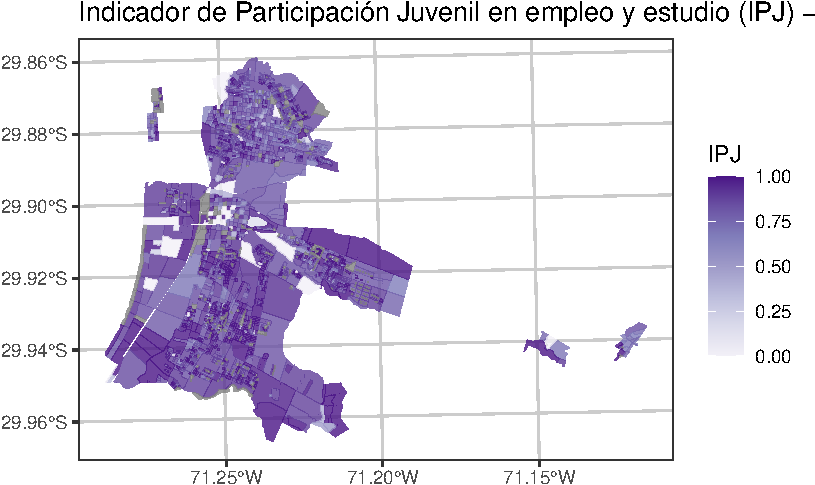
\includegraphics{./datos_vectoriales_files/figure-pdf/fig-ipj-urbano-1.pdf}

}

\caption{\label{fig-ipj-urbano}Indicador de Participación Juvenil
enempleo y estudio (IPJ) - Urbano}

\end{figure}

\begin{Shaded}
\begin{Highlighting}[]
\CommentTok{\# mapview::mapview(la\_serena\_urb, }
\CommentTok{\#                  zcol = "IPJ", layer.name = "IPJ")}
\end{Highlighting}
\end{Shaded}

\hypertarget{indicador-de-resiliencia-de-hogares-irh}{%
\section{Indicador de Resiliencia de Hogares
(IRH)}\label{indicador-de-resiliencia-de-hogares-irh}}

En particular, la monoparentalidad es ampliamente reconocida en la
literatura internacional como una situación familiar frágil, que puede
afectar las trayectorias de vida de los hijos, en términos de un mayor
riesgo de mortalidad (Amato \& Patterson, 2017), inestabilidad
psicológica (Theodoritsi, Daliana \& Antoniou, 2018), problemas de salud
(Duriancik \& Goff, 2019) y otros.

En suma, el Indicador de Resiliencia de Hogares (en base a la
monoparentalidad), en complemento a otras variables, es conceptualmente
relevante para evaluar riesgos no monetarios de condiciones sociales.

Este indicador es el inverso aditivo de la proporción de hogares
monoparentales dentro de una manzana. Los hogares monoparentales son
aquellos con hijos que viven con un solo progenitor, lo que se asocia en
diversas formas a la condición social, que abarcan desde un menor
ingreso, problemas de salud y delincuencia, entre otros (MDS, 2019).

Al contrario, los hogares biparentales permiten el apoyo entre
progenitores y los hogares sin hijos tienen menores exigencias de gasto
y tiempo relacionadas con la paternidad, por lo que se considera que en
general son más resilientes.

** Cáñculo de Indicador de Resiliencia de Hogares (IRH) **

\textbf{MONOPAR}: Hogares Monoparentales\\
\textbf{HOG\_N}: Número de Hogares

\begin{Shaded}
\begin{Highlighting}[]
\NormalTok{censo }\OtherTok{\textless{}{-}}\NormalTok{ censo }\SpecialCharTok{\%\textgreater{}\%} \FunctionTok{mutate}\NormalTok{( }\AttributeTok{MONO\_DENS =}\NormalTok{ MONOPAR }\SpecialCharTok{/}\NormalTok{ HOG\_N)}
\NormalTok{censo }\OtherTok{\textless{}{-}}\NormalTok{ censo }\SpecialCharTok{\%\textgreater{}\%} \FunctionTok{mutate}\NormalTok{( }\AttributeTok{MONO\_DENS =} \FunctionTok{ifelse}\NormalTok{(MONO\_DENS }\SpecialCharTok{\textgreater{}} \DecValTok{1}\NormalTok{, }\DecValTok{1}\NormalTok{, MONO\_DENS))  }
\NormalTok{censo }\OtherTok{\textless{}{-}}\NormalTok{ censo }\SpecialCharTok{\%\textgreater{}\%} \FunctionTok{mutate}\NormalTok{( }\AttributeTok{IRH =} \DecValTok{1} \SpecialCharTok{{-}}\NormalTok{ MONO\_DENS)}
\end{Highlighting}
\end{Shaded}

\begin{Shaded}
\begin{Highlighting}[]
\NormalTok{la\_serena\_urb }\OtherTok{\textless{}{-}}\NormalTok{ censo }\SpecialCharTok{\%\textgreater{}\%} \FunctionTok{filter}\NormalTok{(COD\_COM }\SpecialCharTok{==} \DecValTok{4101} \SpecialCharTok{\&}\NormalTok{ MANZ\_EN }\SpecialCharTok{==} \StringTok{"URBANO"}\NormalTok{)}
\end{Highlighting}
\end{Shaded}

\textbf{Visualizar la Variable de \texttt{IRH} comuna de La Serena
\texttt{URBANO}}:

\begin{Shaded}
\begin{Highlighting}[]
\FunctionTok{ggplot}\NormalTok{() }\SpecialCharTok{+}
  \FunctionTok{geom\_sf}\NormalTok{(}\AttributeTok{data =}\NormalTok{ la\_serena\_urb, }\FunctionTok{aes}\NormalTok{(}\AttributeTok{fill =}\NormalTok{ IRH), }\AttributeTok{color =}\ConstantTok{NA}\NormalTok{, }
          \AttributeTok{alpha=}\FloatTok{0.8}\NormalTok{,  }\AttributeTok{size=} \FloatTok{0.1}\NormalTok{)}\SpecialCharTok{+}
  \FunctionTok{scale\_fill\_distiller}\NormalTok{(}\AttributeTok{palette=} \StringTok{"PuRd"}\NormalTok{, }\AttributeTok{direction =} \DecValTok{1}\NormalTok{)}\SpecialCharTok{+}
  \FunctionTok{ggtitle}\NormalTok{(}\StringTok{"Indicador de Resiliencia de Hogares (IRH) {-} Urbano"}\NormalTok{) }\SpecialCharTok{+}
  \FunctionTok{theme\_bw}\NormalTok{() }\SpecialCharTok{+}
  \FunctionTok{theme}\NormalTok{(}\AttributeTok{panel.grid.major =} \FunctionTok{element\_line}\NormalTok{(}\AttributeTok{colour =} \StringTok{"gray80"}\NormalTok{), }
        \AttributeTok{panel.grid.minor =} \FunctionTok{element\_line}\NormalTok{(}\AttributeTok{colour =} \StringTok{"gray80"}\NormalTok{))}
\end{Highlighting}
\end{Shaded}

\begin{figure}[H]

{\centering 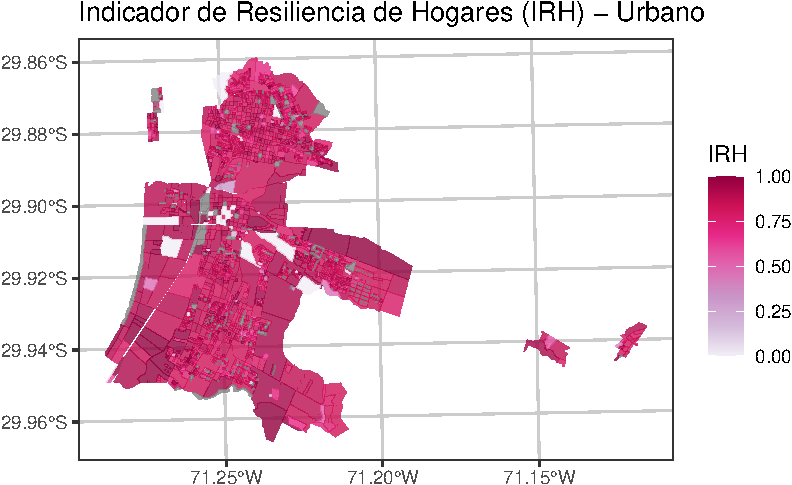
\includegraphics{./datos_vectoriales_files/figure-pdf/fig-irh-urbano-1.pdf}

}

\caption{\label{fig-irh-urbano}Indicador de Resiliencia de Hogares (IRH)
- Urbano}

\end{figure}

\begin{Shaded}
\begin{Highlighting}[]
\CommentTok{\# mapview::mapview(la\_serena\_urb, }
\CommentTok{\#                  zcol = "IRH", layer.name = "IRH")}
\end{Highlighting}
\end{Shaded}

\hypertarget{indicador-de-calidad-de-la-vivienda-ivi}{%
\section{Indicador de Calidad de la Vivienda
(IVI)}\label{indicador-de-calidad-de-la-vivienda-ivi}}

El indicador de calidad de vivienda es una variable sintética de todas
las materialidades de la vivienda. Inicialmente, se construyó como un
indicador de mala calidad, tomando un valor más alto cuando la calidad
de la vivienda es peor y es más bajo cuando es mejor. Fue elaborado como
un promedio lineal del 3 sub-indicadores de paredes, suelo y techo. Cada
uno de estos sub-indicadores registra el porcentaje de viviendas de la
manzana que tienen paredes, suelo o techo considerado insuficiente. Las
construcciones consideradas insuficientes son las siguientes:

\textbf{Paredes}: Material de los muros exteriores

\begin{itemize}
\tightlist
\item
  P03A\_4: Tabique sin forro interior (madera u otro)
\item
  P03A\_5: Adobe, barro, quincha, pirca u otro artesanal tradicional
\item
  P03A\_6: Materiales precarios (lata, cartón, plástico, etc.)
\end{itemize}

\textbf{Techo}: Material en la cubierta del techo

\begin{itemize}
\tightlist
\item
  P03B\_4: Fonolita o plancha de fieltro embreado
\item
  P03B\_6: Materiales precarios (lata, cartón, plásticos, etc.)
\item
  P03B\_7: Sin cubierta sólida de techo
\end{itemize}

\textbf{Suelo}: Material de construcción del piso

\begin{itemize}
\tightlist
\item
  P03C\_4: Capa de cemento sobre tierra
\item
  P03C\_5: Tierra
\end{itemize}

** Cálculo Indicador de Calidad de la Vivienda (IVI) **

\begin{Shaded}
\begin{Highlighting}[]
\NormalTok{censo }\OtherTok{\textless{}{-}}\NormalTok{ censo }\SpecialCharTok{\%\textgreater{}\%}
  \FunctionTok{mutate}\NormalTok{(}\AttributeTok{paredes =}\NormalTok{ (P03A\_4 }\SpecialCharTok{+}\NormalTok{ P03A\_5 }\SpecialCharTok{+}\NormalTok{ P03A\_6)}\SpecialCharTok{/}\NormalTok{TOTAL\_V,}
         \AttributeTok{techo =}\NormalTok{ (P03B\_4 }\SpecialCharTok{+}\NormalTok{ P03B\_6 }\SpecialCharTok{+}\NormalTok{ P03B\_7)}\SpecialCharTok{/}\NormalTok{TOTAL\_V,}
         \AttributeTok{suelo =}\NormalTok{ (P03C\_4 }\SpecialCharTok{+}\NormalTok{  P03C\_5)}\SpecialCharTok{/}\NormalTok{TOTAL\_V)}

\CommentTok{\# eliminar valores infinitos de la división anterior}
\NormalTok{censo }\OtherTok{\textless{}{-}}\NormalTok{ censo }\SpecialCharTok{\%\textgreater{}\%}
  \FunctionTok{mutate}\NormalTok{(}\AttributeTok{paredes =} \FunctionTok{ifelse}\NormalTok{(paredes }\SpecialCharTok{\textgreater{}} \DecValTok{1}\NormalTok{, }\DecValTok{1}\NormalTok{, paredes), }
         \AttributeTok{techo =} \FunctionTok{ifelse}\NormalTok{(techo }\SpecialCharTok{\textgreater{}} \DecValTok{1}\NormalTok{, }\DecValTok{1}\NormalTok{, techo), }
         \AttributeTok{suelo =} \FunctionTok{ifelse}\NormalTok{(suelo }\SpecialCharTok{\textgreater{}} \DecValTok{1}\NormalTok{, }\DecValTok{1}\NormalTok{, suelo))}

\NormalTok{censo }\OtherTok{\textless{}{-}}\NormalTok{ censo }\SpecialCharTok{\%\textgreater{}\%}  \FunctionTok{mutate}\NormalTok{(}\AttributeTok{IVI =}\NormalTok{ (paredes}\SpecialCharTok{+}\NormalTok{ suelo}\SpecialCharTok{+}\NormalTok{ techo)}\SpecialCharTok{/}\DecValTok{3}\NormalTok{)}
\NormalTok{censo }\OtherTok{\textless{}{-}}\NormalTok{ censo }\SpecialCharTok{\%\textgreater{}\%}  \FunctionTok{mutate}\NormalTok{(}\AttributeTok{IVI =}  \DecValTok{1} \SpecialCharTok{{-}}\NormalTok{ IVI) }\CommentTok{\# invertir sentido}
\end{Highlighting}
\end{Shaded}

\begin{Shaded}
\begin{Highlighting}[]
\NormalTok{la\_serena\_urb }\OtherTok{\textless{}{-}}\NormalTok{ censo }\SpecialCharTok{\%\textgreater{}\%} \FunctionTok{filter}\NormalTok{(COD\_COM }\SpecialCharTok{==} \DecValTok{4101} \SpecialCharTok{\&}\NormalTok{ MANZ\_EN }\SpecialCharTok{==} \StringTok{"URBANO"}\NormalTok{)}
\end{Highlighting}
\end{Shaded}

\textbf{Visualizar la Variable de \texttt{IVI} comuna de La Serena
\texttt{URBANO}}:

\begin{Shaded}
\begin{Highlighting}[]
\FunctionTok{ggplot}\NormalTok{() }\SpecialCharTok{+}
  \FunctionTok{geom\_sf}\NormalTok{(}\AttributeTok{data =}\NormalTok{ la\_serena\_urb, }\FunctionTok{aes}\NormalTok{(}\AttributeTok{fill =}\NormalTok{ IVI), }\AttributeTok{color =}\ConstantTok{NA}\NormalTok{, }
          \AttributeTok{alpha=}\FloatTok{0.8}\NormalTok{,  }\AttributeTok{size=} \FloatTok{0.1}\NormalTok{)}\SpecialCharTok{+}
  \FunctionTok{scale\_fill\_distiller}\NormalTok{(}\AttributeTok{palette=} \StringTok{"YlOrRd"}\NormalTok{, }\AttributeTok{direction =} \DecValTok{1}\NormalTok{)}\SpecialCharTok{+}
  \FunctionTok{ggtitle}\NormalTok{(}\StringTok{"Indicador de Calidad de la Vivienda (IVI) {-} Urbano"}\NormalTok{) }\SpecialCharTok{+}
  \FunctionTok{theme\_bw}\NormalTok{() }\SpecialCharTok{+}
  \FunctionTok{theme}\NormalTok{(}\AttributeTok{panel.grid.major =} \FunctionTok{element\_line}\NormalTok{(}\AttributeTok{colour =} \StringTok{"gray80"}\NormalTok{), }
        \AttributeTok{panel.grid.minor =} \FunctionTok{element\_line}\NormalTok{(}\AttributeTok{colour =} \StringTok{"gray80"}\NormalTok{))}
\end{Highlighting}
\end{Shaded}

\begin{figure}[H]

{\centering 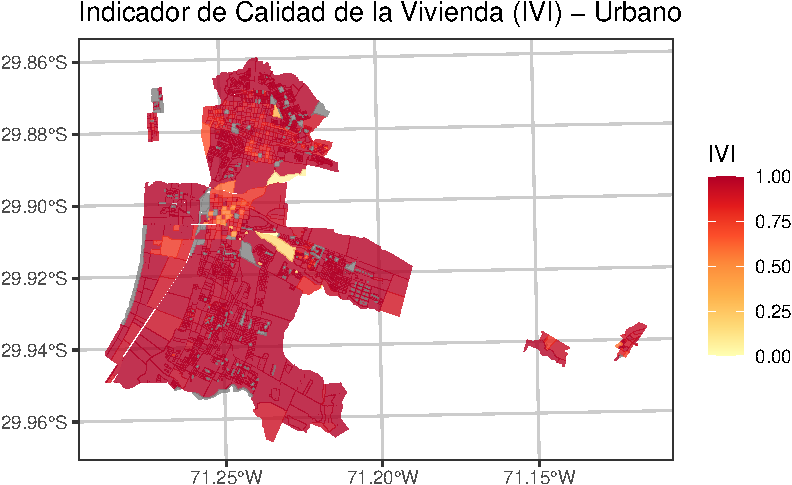
\includegraphics{./datos_vectoriales_files/figure-pdf/fig-ivi-urbano-1.pdf}

}

\caption{\label{fig-ivi-urbano}Indicador de Calidad de la Vivienda (IVI)
- Urbano}

\end{figure}

\begin{Shaded}
\begin{Highlighting}[]
\CommentTok{\# mapview::mapview(la\_serena\_urb, }
\CommentTok{\#                  zcol = "IVI", layer.name = "IVI")}
\end{Highlighting}
\end{Shaded}

\hypertarget{indicador-de-suficiencia-de-viviendas-isv}{%
\section{Indicador de Suficiencia de Viviendas
(ISV)}\label{indicador-de-suficiencia-de-viviendas-isv}}

El indicador de Suficiencia de Viviendas se construyó inicialmente como
un indicador de hacinamiento. Se realizó a partir de 2 variables que
indican el número de viviendas que se encuentran en situación de
hacinamiento y el número de viviendas que se encuentran en situación de
hacinamiento severo. El indicador corresponde a la suma de 2 veces las
viviendas en situación de hacinamiento severo con las viviendas en
situación de hacinamiento normal, dividido por el total de viviendas.

Luego, el indicador se normalizó con su inverso aditivo, para asegurar
que el valor máximo, sea lo más deseable y el 0 lo menos deseable. Con
esto se obtuvo el indicador de suficiencia de viviendas.

\textbf{Cálculo de Indicador de Suficiencia de Viviendas (ISV) }

\textbf{NIV\_HAC2}: \textgreater= 2.5 personas por habitación\\
\textbf{NIV\_HAC3}: \textgreater= 5 personas por habitación

\begin{Shaded}
\begin{Highlighting}[]
\NormalTok{censo }\OtherTok{\textless{}{-}}\NormalTok{ censo }\SpecialCharTok{\%\textgreater{}\%} \FunctionTok{mutate}\NormalTok{(}\AttributeTok{ISV =}\NormalTok{ NIV\_HAC2 }\SpecialCharTok{+}\NormalTok{ (}\DecValTok{2} \SpecialCharTok{*}\NormalTok{ NIV\_HAC3))}

\CommentTok{\# función de normalización}
\NormalTok{minmax }\OtherTok{\textless{}{-}} \ControlFlowTok{function}\NormalTok{(x) \{}
\NormalTok{  x }\OtherTok{\textless{}{-}}\NormalTok{ (x }\SpecialCharTok{{-}} \FunctionTok{min}\NormalTok{(x, }\AttributeTok{na.rm =} \ConstantTok{TRUE}\NormalTok{)) }\SpecialCharTok{/} 
\NormalTok{    (}\FunctionTok{max}\NormalTok{(x, }\AttributeTok{na.rm =} \ConstantTok{TRUE}\NormalTok{) }\SpecialCharTok{{-}} \FunctionTok{min}\NormalTok{(x, }\AttributeTok{na.rm =} \ConstantTok{TRUE}\NormalTok{))}
  \FunctionTok{return}\NormalTok{(x)}
\NormalTok{\}}

\NormalTok{censo }\OtherTok{\textless{}{-}}\NormalTok{ censo }\SpecialCharTok{\%\textgreater{}\%} \FunctionTok{mutate}\NormalTok{(}\AttributeTok{ISV =} \DecValTok{1} \SpecialCharTok{{-}} \FunctionTok{minmax}\NormalTok{(ISV))}
\end{Highlighting}
\end{Shaded}

\begin{Shaded}
\begin{Highlighting}[]
\NormalTok{la\_serena\_urb }\OtherTok{\textless{}{-}}\NormalTok{ censo }\SpecialCharTok{\%\textgreater{}\%} \FunctionTok{filter}\NormalTok{(COD\_COM }\SpecialCharTok{==} \DecValTok{4101} \SpecialCharTok{\&}\NormalTok{ MANZ\_EN }\SpecialCharTok{==} \StringTok{"URBANO"}\NormalTok{)}
\end{Highlighting}
\end{Shaded}

\textbf{Visualizar la Variable de \texttt{ISV} comuna de La Serena
\texttt{URBANO}}:

\begin{Shaded}
\begin{Highlighting}[]
\FunctionTok{ggplot}\NormalTok{() }\SpecialCharTok{+}
  \FunctionTok{geom\_sf}\NormalTok{(}\AttributeTok{data =}\NormalTok{ la\_serena\_urb, }\FunctionTok{aes}\NormalTok{(}\AttributeTok{fill =}\NormalTok{ ISV), }\AttributeTok{color =}\ConstantTok{NA}\NormalTok{, }
          \AttributeTok{alpha=}\FloatTok{0.8}\NormalTok{,  }\AttributeTok{size=} \FloatTok{0.1}\NormalTok{)}\SpecialCharTok{+}
  \FunctionTok{scale\_fill\_distiller}\NormalTok{(}\AttributeTok{palette=} \StringTok{"YlOrRd"}\NormalTok{, }\AttributeTok{direction =} \DecValTok{1}\NormalTok{)}\SpecialCharTok{+}
  \FunctionTok{ggtitle}\NormalTok{(}\StringTok{" Indicador de Suficiencia de Viviendas (ISV) {-} Urbano"}\NormalTok{) }\SpecialCharTok{+}
  \FunctionTok{theme\_bw}\NormalTok{() }\SpecialCharTok{+}
  \FunctionTok{theme}\NormalTok{(}\AttributeTok{panel.grid.major =} \FunctionTok{element\_line}\NormalTok{(}\AttributeTok{colour =} \StringTok{"gray80"}\NormalTok{), }
        \AttributeTok{panel.grid.minor =} \FunctionTok{element\_line}\NormalTok{(}\AttributeTok{colour =} \StringTok{"gray80"}\NormalTok{))}
\end{Highlighting}
\end{Shaded}

\begin{figure}[H]

{\centering 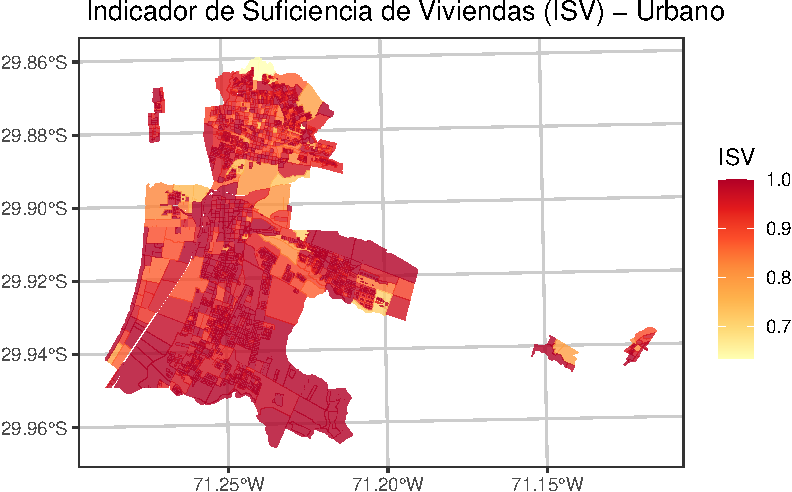
\includegraphics{./datos_vectoriales_files/figure-pdf/fig-isv-urbano-1.pdf}

}

\caption{\label{fig-isv-urbano}Indicador de Suficiencia de Viviendas
(ISV) - Urbano}

\end{figure}

\begin{Shaded}
\begin{Highlighting}[]
\CommentTok{\# mapview::mapview(la\_serena\_urb, }
\CommentTok{\#                  zcol = "ISV", layer.name = "ISV")}
\end{Highlighting}
\end{Shaded}

\hypertarget{consolidaciuxf3n-de-dimensiuxf3n-socioeconuxf3mica}{%
\section{Consolidación de Dimensión
Socioeconómica}\label{consolidaciuxf3n-de-dimensiuxf3n-socioeconuxf3mica}}

\textbf{Selección de Variables de Interés}

\begin{Shaded}
\begin{Highlighting}[]
\CommentTok{\# names(censo)}
\NormalTok{soc }\OtherTok{\textless{}{-}}\NormalTok{ censo }\SpecialCharTok{\%\textgreater{}\%} 
\NormalTok{  dplyr}\SpecialCharTok{::}\FunctionTok{select}\NormalTok{(ID\_MANZ}\SpecialCharTok{:}\NormalTok{PERSONAS, IEJ, IEM, IPJ, IRH, IVI, ISV)}
\end{Highlighting}
\end{Shaded}

\textbf{Visualización de los Indicadores}

\begin{Shaded}
\begin{Highlighting}[]
\NormalTok{comuna }\OtherTok{\textless{}{-}}\NormalTok{ soc }\SpecialCharTok{\%\textgreater{}\%} \FunctionTok{filter}\NormalTok{(COD\_COM }\SpecialCharTok{==} \DecValTok{4101} \SpecialCharTok{\&}\NormalTok{ MANZ\_EN }\SpecialCharTok{==} \StringTok{"URBANO"}\NormalTok{)}
\FunctionTok{mapview}\NormalTok{(comuna, }\AttributeTok{zcol =} \StringTok{"IEJ"}\NormalTok{) }\SpecialCharTok{+} \FunctionTok{mapview}\NormalTok{(comuna, }\AttributeTok{zcol =} \StringTok{"IEM"}\NormalTok{)}\SpecialCharTok{+}
  \FunctionTok{mapview}\NormalTok{(comuna, }\AttributeTok{zcol =} \StringTok{"IPJ"}\NormalTok{) }\SpecialCharTok{+} \FunctionTok{mapview}\NormalTok{(comuna, }\AttributeTok{zcol =} \StringTok{"IRH"}\NormalTok{)}\SpecialCharTok{+}
  \FunctionTok{mapview}\NormalTok{(comuna, }\AttributeTok{zcol =} \StringTok{"IVI"}\NormalTok{) }\SpecialCharTok{+} \FunctionTok{mapview}\NormalTok{(comuna, }\AttributeTok{zcol =} \StringTok{"ISV"}\NormalTok{)}
\end{Highlighting}
\end{Shaded}

\textbf{Guardar Resultados}

\begin{Shaded}
\begin{Highlighting}[]
\CommentTok{\# guardar shapefile}
\NormalTok{path\_file\_out }\OtherTok{\textless{}{-}} \FunctionTok{paste0}\NormalTok{(}\StringTok{"../data/socioeconomicos/resultados/"}\NormalTok{,}
\NormalTok{                    reg, }\StringTok{"\_ind\_socioeconomicos.shp"}\NormalTok{)}
\FunctionTok{st\_write}\NormalTok{(soc, path\_file\_out)}

\CommentTok{\#guardar en RDS}
\NormalTok{path\_file\_out\_rds }\OtherTok{\textless{}{-}} \FunctionTok{paste0}\NormalTok{(}\StringTok{"../data/socioeconomicos/resultados/"}\NormalTok{,}
\NormalTok{                    reg, }\StringTok{"\_ind\_socioeconomicos.rds"}\NormalTok{)}
\FunctionTok{saveRDS}\NormalTok{(soc, path\_file\_out\_rds)  }
\end{Highlighting}
\end{Shaded}

\hypertarget{referencias-1}{%
\section{Referencias}\label{referencias-1}}

\begin{itemize}
\tightlist
\item
  \href{https://es.r4ds.hadley.nz}{R para Ciencia de Datos}
\item
  \href{https://bookdown.org/gboccardo/manual-ED-UCH/}{RStudio para
  Estadística Descriptiva en Ciencias Sociales}
\item
  \href{https://bookdown.org/jboscomendoza/r-principiantes4/}{R para
  Principiantes4/}
\item
  \href{https://ggplot2-book.org/scale-colour.html}{Colores en Ggplot2}
\end{itemize}

\bookmarksetup{startatroot}

\hypertarget{references}{%
\chapter*{References}\label{references}}
\addcontentsline{toc}{chapter}{References}

\hypertarget{refs}{}
\begin{CSLReferences}{0}{0}
\end{CSLReferences}



\end{document}
